%% -----------------------------------------------------------------
%%  Original Template
%% -----------------------------------------------------------------
%%
%%   Author:    Tim Callagha, University of Tasmania (UTas)
%%   Email:     tgc@hilbert.maths.utas.edu.au
%%   Copyright: 2003 Tim Callagha
%% 
%%   Style file to assist in generating a University of Tasmania PhD thesis
%%   in Mathematics. Contains all the required formatting options and 
%%   header/footer information that is set out in the Research Higher Degrees 
%%   Resource Handbook (2003 version)
%%
%%   This file should be easily modifiable to comply with
%%   minor formatting changes (such as the left margin width etc.)
%% 
%%   This style file is designed primarily for students of mathematics at UTas who
%%   are undertaking a PhD. However, only very minor changes need to be made to the 
%%   wording in a few places to use it as a template for an honours or Masters thesis 
%%   as well. In fact, there is no particular reason why this could be not used for, 
%%   say, an Arts thesis (Shock, Horror!) since it is mainly about the formatting and 
%%   less about the content. However, the heading and chapter structure has been chosen
%%   so as to be more in line with standard practice in the scientific streams. Again, 
%%   if you know what you're doing then it's really not that difficult to modify the style 
%%   file at the appropriate places. I have tried to comment it quite heavily so that 
%%   interested persons can see how it does all its work and, hopefully, make changes 
%%   that reflect personal tastes etc.
%%
%%   Source: http://staff.acecrc.org.au/~mdsumner/TCallaghan/
%% 
%%   This work consists of the files listed in the README file.
%%
%% -----------------------------------------------------------------
%%  Modifications for Australian Maritime College (AMC) and
%%	University of Tasmania (UTas) Department of Engineering 
%% -----------------------------------------------------------------
%%
%%   Author:  Konrad Zürcher, Australian Maritime College (AMC)
%%   Email:   Konrad.Zurcher@utas.edu.au
%%   License: MIT License
%%
%%	 Modified version of the original template adjusted for styling
%%   requirements of the University of Tasmania (UTas) Department of 
%%   Engineering and the Australian Maritime College (AMC).
%%
%%   GitHub: https://github.com/SeaShadow/LaTeX-AMC-PhD-Template
%% 
%%   This work consists of the files listed in the README file.
%%
%% -----------------------------------------------------------------
%%

% thesis.tex (starting point of a UTas mathematics thesis)

% Note that the following defaults are also contained in the 'report' class
% (this is not exhaustive...see appropriate references for all options)
% 'oneside' mode...overide with 'twoside' to force output for two-sided printing.
% 'final' mode...overide with 'draft' to see linebreak malfunctioning.
% For example, to use two-sided printing one would declare the 'documentclass'
% as follows...
% '\documentclass[11pt,a4paper,twoside]{report}'
%
% Specific Mathematical options are as follows
% 'leqno' to force equation numbering on the left side of the page.
% 'fleqn' to force formulas to flush left (centered is the default).
% If 'fleqn' is specified then the left indent is controlled with '\mathindent'.
% i.e. '\setlength{\mathindent}{2.5cm}'

% Declare overall type of document (use 11pt report class on A4 paper).
\documentclass[11pt,a4paper,final]{report}

% If you want to generate an index you should include the following command
% which puts a makeindex command in the preamble. Additionally, you need to un-comment
% the file 'index' in the '\includeonly' command below and also include the 'index'
% file in the main document.
\makeindex
\PassOptionsToPackage{nottoc}{tocbibind}

% Include the style file which contains all the required formatting
% information that is set out in the Research Higher Degrees Resource
% Handbook (2003 version). NOTE: This file uses the following packages
% 'graphicx' for graphics manipulation
% 'fancyhdr' for nice headers and footers.
% 'makeidx' for generating the index
% 'tocbibind' for adding table of contents entries for bibliography, index etc.
% 'sectsty' for generating stylised chapter and section headings.
% 'lipsum' for generating dummy text.
% 'natbib' and 'har2nat' for bib citations.
% 'xcolor' color package.
% 'epstopdf' EPS to PDF conversion.
% You will need to make sure your LaTeX installation has these packages
% installed...else it wont work :(
\usepackage{Packages/mathphdthesis}

% acro package for acronims
\usepackage{acro}

\DeclareAcronym{2d}{
	short=2D,
	long=two-dimensional,
}
\DeclareAcronym{3d}{
	short=3D,
	long=three-dimensional,
}
\DeclareAcronym{a0}{
	short=A$_0$,
	long=antisymmetric fundamental Lamb wave mode,
}
\DeclareAcronym{ccd}{
	short=CCD,
	long=correlation coefficient deviation,
}
\DeclareAcronym{cfrp}{
	short=CFRP,
	long=carbon fiber reinforced polymer,
}
\DeclareAcronym{di}{
	short=DI,
	long=damage index,
}
\DeclareAcronym{dau}{
	short=DAU,
	long=data acquisition unit,
}
\DeclareAcronym{dof}{
	short=DOF,
	long=degree of freedom,
}
\DeclareAcronym{emi}{
	short=EMI,
	long=electromechanical impedance,
}
\DeclareAcronym{fem}{
	short=FEM,
	long=finite element method,
}
\DeclareAcronym{fbg}{
	short=FBG,
	long=fiber Bragg grating,
}
\DeclareAcronym{gw}{
	short=GW,
	long=guided waves,
}
\DeclareAcronym{gll}{
	short=GLL,
	long=Gauss-Lobatto-Legendre,
}
\DeclareAcronym{gpu}{
	short=GPU,
	long=graphics processing unit,
}
\DeclareAcronym{hsc}{
	short=HSC,
	long=honeycomb sandwich composite,
}
\DeclareAcronym{ncn}{
	short=NCN,
	long=National Science Centre,
}
\DeclareAcronym{madif}{
	short=MADIF,
	long=model assisted damage identification function,
}
\DeclareAcronym{mapd}{
	short=MAPD,
	long=mean absolute percentage deviation,
}
\DeclareAcronym{pnn}{
	short=PNN,
	long=probabilistic neural networks,
}
\DeclareAcronym{pzt}{
	short=PZT,
	long=piezoelectric transducer,
}
\DeclareAcronym{rms}{
	short=RMS,
	long=root mean square,
}
\DeclareAcronym{rmsd}{
	short=RMSD,
	long=root mean square deviation,
}
\DeclareAcronym{rve}{
	short=RVE,
	long=representative volume element,
}
\DeclareAcronym{s0}{
	short=S$_0$,
	long=symmetric fundamental Lamb wave mode,
}
\DeclareAcronym{sem}{
	short=SEM,
	long=spectral element method,
}
\DeclareAcronym{scs}{
	short=SCS,
	long=sandwich composite structure,
}
\DeclareAcronym{shm}{
	short=SHM,
	long=structural health monitoring,
}
\DeclareAcronym{sldv}{
	short=SLVD,
	long=scanning laser Doppler vibrometer,
}

\usepackage[ruled,vlined]{algorithm2e}
\usepackage{multirow}
\graphicspath{{Figures/}} %Setting the graphicspath
% Here you would include any additional packages that you want to use.
% You should make sure they don't clash with the above packages that
% are in use in the style file.

% Specify which pieces (other .tex files) you plan to include. You can comment
% out files that you will include later or have already finished to speed
% up TeX processing
\includeonly{
Frontbackmatter/prelude 	% Contains all the relevant candidate information (name, degrees, abstract etc)
,Frontbackmatter/newcom 	% Place all you new commands in here
,Nomenclature/nomenclature  % The nomenclature chapter
,Acronyms/acronyms			% Acronyms chapter
,Chapters/Intro/intro  	    % The first chapter
,Chapters/Chapter2/ch:problem 	% Chp2
,Chapters/Chapter3/ch:method 	% Chp3
,Chapters/Chapter4/ch:sem 		% Chp4
,Chapters/Chapter5/ch:simulation 		% Chp5
,Chapters/Chapter6/ch:validation 	% Chp6
,Chapters/Chapter7/ch:tempEffect 	% Chp7
,Chapters/Chapter8/ch:severity 	% Ch8
,Chapters/Chapter9/ch:conclusions	% Chp9
,Appendices/app0   			% Needed to switch to appendix mode
,index  					% Places the index in the thesis
}

% Begin the thesis
\begin{document}

% Include all the pieces of your thesis in here
% prelude.tex (specification of which features in `mathphdthesis.sty' you
% are using, your personal information, and your title & abstract)

% Specify features of `mathphdthesis.sty' you want to use:
\titlepgtrue 												% Main title page (required)
\signaturepagetrue 											% Page for declaration of originality (required)
\copyrighttrue 												% Copyright page (required)
\abswithesistrue 											% Abstract to be bound with thesis (optional)
\acktrue 													% Acknowledgments page (optional)
\tablecontentstrue 											% Table of contents page (required)
\tablespagetrue 											% Table of contents page for tables (required only if you have tables)
\figurespagetrue 											% Table of contents page for figures (required only if you have figures)

% Title, author, supervisors, university, date of submission
\title{Modelling of sandwich plates and piezoelectric transducers to identify the severity of mechanical damage}							% Thesis title
\author{Piotr Fiborek} 	% First name and surname of candidate (e.g. John Doe)
\prevdegrees{M.Sc. Eng.}              			% Specify your previous degrees (e.g. B.E. (Hons))
\institute{Mechanics of Intelligent Structures Department}								% Institute of department (e.g. National Centre for Maritime Engineering and Hydrodynamics)

\submittedfor{A dissertation submitted to the Scientific Board of the Szewalski Institute of Fluid Flow Machinery, Polish Academy of Sciences in partial fulfillment of the requirements for the Degree of Doctor of Philosophy}			% Degree thesis is submitted for (e.g. Submitted in fulfillment of the requirements for the Degree of Doctor of Philosophy)
\advisor{ Pawe\l{} Kudela, D.Sc. Ph.D. Eng.} % Supervisors: (e.g. Prof. Lawrence K. Forbes)
\dept{The Szewalski Institute of Fluid Flow Machinery, Polish Academy of Sciences}
\submitdate{June, 2022}						% Month & year of your thesis submission (e.g. January, 2016)

% Abstract to be bound with thesis
\newcommand{\abstextwithesis}
{
%Basic abstract goes here. Can use paragraphs and normal \LaTeX commands.
...
}

% Acknowledgments page
\newcommand{\acknowledgement}
{
}

% Engineering guote page
\newcommand{\engineeringquote}
{
\null\vskip1.8in
\begin{quote}
"Engineering ."\begin{flushright}- aaa 
\end{flushright}
\end{quote}
}

% Bibliography Title
\renewcommand{\bibname}{Bibliography}
% Bibliography spacing
\setlength\bibitemsep{1.5\itemsep}

% Settings for array package
\newcolumntype{L}[1]{>{\raggedright\let\newline\\\arraybackslash\hspace{0pt}}m{#1}}
\newcolumntype{C}[1]{>{\centering\let\newline\\\arraybackslash\hspace{0pt}}m{#1}}
\newcolumntype{R}[1]{>{\raggedleft\let\newline\\\arraybackslash\hspace{0pt}}m{#1}}

% Take care of things in `mathphdthesis.sty' behind the scenes.
% Basically just does a check of all the fields that have been activated
% above and fills out the appropriate pages and adds them to the thesis.
\beforepreface
\afterpreface

% newcom.tex (new command definitions)

% Some examples (yours may be different):
\newtheorem{theorem}{Theorem}[section]
\newtheorem{lemma}[theorem]{Lemma}
\newcommand{\bfx}{{\ensuremath{\mathbf{x}}}}

% chap9.tex (Chapter 9 of the thesis)

%\chapter[NOMENCLATURE]{NOMENCLATURE}
% Overwrite TOC chapter title
\chapter*{NOMENCLATURE}
\addcontentsline{toc}{chapter}{NOMENCLATURE}
\label{nomenclature}

% -----------------------------------------------------------------------------------------------------------------
% Greek symbols
% -----------------------------------------------------------------------------------------------------------------

% GENERAL CONSTANTS

% -----------------------------------------------------------------------------------------------------------------
% Dimensionless numbers
% -----------------------------------------------------------------------------------------------------------------


% -----------------------------------------------------------------------------------------------------------------
% Roman symbols
% -----------------------------------------------------------------------------------------------------------------

% AREAS 
% DIMENSIONS
\printnomenclature[6em]
%\printnomenclature[2cm]

% chap9.tex (Chapter 9 of the thesis)

%\chapter[ACRONYMS]{ACRONYMS}
% Overwrite TOC chapter title
\chapter*{Acronyms}
\addcontentsline{toc}{chapter}{Acronyms}
\label{acronyms}
\printacronyms[heading=none,pages={display=first}]
% Set page numbering to arabic the first time we commence a chapter.
% This is required to get the page numbering correct.
\pagenumbering{arabic}

% Note that the text in the [] brackets is the one that will
% appear in the table of contents, whilst the text in the {}
% brackets will appear in the main thesis.

%% CHAPTER HEADER /////////////////////////////////////////////////////////////////////////////////////
\chapter[Introduction]{Introduction}
\label{ch:intro}
The dissertation is the result of the author’s work as an assistant in the Department of Mechanics of Intelligent Structures, Institute of Fluid Flow Machinery, Polish Academy of Sciences.
Most of the work was carried out within the framework of a research project titled ‘Model-assisted damage identification function for Structural Health Monitoring of composite structures under a varied environmental condition', which was granted to the author by the National Science Centre, Poland.
The primary objective was to develop a new approach to a sandwich structure assessment based on guided waves techniques under varied operating conditions.
The essence of the proposed method was to establish an accurate and numerically efficient model of the wave propagation in the sandwich structure, which allowed for determining the mechanical damage severity.
A better understanding of guided wave behaviour in such structures and their interaction with damage may allow the development of more precise structural health monitoring strategies, reducing costs without compromising the safety of the liable systems.
%% CHAPTER INTRODUCTION ///////////////////////////////////////////////////////////////////////////////

%% INCLUDE SECTIONS ///////////////////////////////////////////////////////////////////////////////////
%% SECTION HEADER /////////////////////////////////////////////////////////////////////////////////////
\section{Sandwich Composite Structures}
\label{sec:scs}

%% SECTION CONTENT ////////////////////////////////////////////////////////////////////////////////////
Composites consist of two or more different materials, such as plastics, resins, metal alloys, glass, carbon or bio-based fibres. The combination of material constituents gives  structure benefits from the properties of the component materials, e.g., the strength of carbon fibres and the low density of the polymer resin in the case of \ac{cfrp}.
The contribution of lightweight composite materials to the production of structural components has been increasing rapidly since the middle of the last century.
Due to the high strength-to-weight ratio, higher operating temperatures, greater stiffness and higher
reliability, composite materials are extensively used in the aircraft and aerospace industry and civil constructions.
Composites account for more than 50\% of the total weight of the aircraft Boeing B787 and Airbus A350 \cite{giurgiutiu2015structural}.

One group of composites includes sandwich panels, which is a type of multi-layered structure that are composed of the mid-core sandwiched between thin skins.
The skins, made of high strength materials, are designed to carry tensile or compressive stresses from longitudinal forces and bending moments.
On the other hand, the core transmits mainly shear stresses from transverse forces.
It also separates the skins, which increases structural stiffness for thin layers, improves insulation properties, and reduces weight while maintaining strength properties similar to the solid construction of the same density.
A popular core used in engineering structures is a honeycomb geometry core.
Fig.~\ref{fig:hcp} shows the construction of the \ac{hsc}.
The core can be made of aluminium, cardboard or Nomex. 
\begin{figure}[H] %hbtp
	\begin{center}
		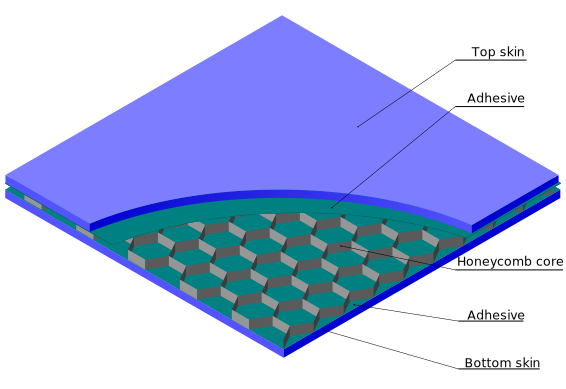
\includegraphics{Intro/honeycomb_plate}
		\caption{
			\label{fig:hcp} Structure of the honeycomb sandwich composite.}
		\vspace{-0.5cm}
	\end{center}
\end{figure}

However, these complex structures are exposed to various types of damage that are not found in metal alloy materials, e.g., hidden disbonds between the skin and the core, delamination of the composite skins, or the core impact damage.
They can occur either during a manufacturing process, storage or in-service life.
Therefore, advanced methods are required for online damage detection.
Thus, the use of composites has forced the development of advanced approaches to structural inspections, e.g., methods based on elastic wave propagation had to account for the anisotropic structure of the material.
%% SECTION HEADER /////////////////////////////////////////////////////////////////////////////////////
\section{Structural health monitoring}
\label{sec:scm}

%% SECTION CONTENT ////////////////////////////////////////////////////////////////////////////////////
\Ac{shm} is the process of implementing an advanced damage identification strategy for structural or mechanical systems \cite{farrar2007introduction}.
The \ac{shm} systems usually consist of a sensor network, a \ac{dau}, and a central processor.
The \ac{dau} is responsible for collecting the data measured by the sensor network.
A central unit then determines the current state of the structure through signal processing and statistical classification.
The implementation of \ac{shm} aims to extend the safe life of the monitored system, or usage of lightweight materials, which leads to cost reduction in production and operation.
For example, composites and adhesive bonding techniques reduces the aircraft's overall weight, reducing fuel consumption \cite{scelsi2011potential}.
\ac{shm} is most commonly found in structures, such as aerospace, civil and mechanical engineering, where damage can have catastrophic consequences.

Rytter, in his dissertation \cite{rytter1993vibrational}, classified the \ac{shm} system advancement into the following four levels:
\begin{itemize}
	\item[] \textbf{Level 1}: Detection.
	\item[] \textbf{Level 2}: Localization.
	\item[] \textbf{Level 3}: Assessment.
	\item[] \textbf{Level 4}: Consequence.
\end{itemize}
The first level determines if any adverse change in the geometric has occurred or material characteristics of the system. The second level leads to the localization of the damage.
The third and fourth level systems determine the size of the flaw and decide whether any maintenance is necessary, respectively.
The existence and location of faults can be defined in unsupervised learning mode by taking a threshold value for a measurable, damage-sensitive system feature. The threshold should be compensated depending on the prevailing operational and environmental conditions.
In contrast, damage size is determined in supervised learning mode based on an analytical model or data extracted experimentally from the structure \cite{worden2007fundamental}.
%% SECTION HEADER /////////////////////////////////////////////////////////////////////////////////////
\section{Piezoelectric Transducers}
\label{sec:challenges}

%% SECTION CONTENT ////////////////////////////////////////////////////////////////////////////////////


%% SECTION HEADER /////////////////////////////////////////////////////////////////////////////////////
\section{Chosen \ac{shm} techniques using \acp{pzt}}
\label{sec:techniques}

%% SECTION CONTENT ////////////////////////////////////////////////////////////////////////////////////

\subsection{Guided waves based techniques}


\Acp{gw} are mechanical vibrations being a superposition of shear and longitudinal waves propagating in a bounded elastic medium, e.g., bars, beams, rods, plates and shells. 
Guided waves are multi-modal and dispersive, i.e. more than one mode travels simultaneously through the medium with the phase velocity depending on the frequency.
Fig.~\ref{fig:dispersion} shows an example of dispersion curves generated by the Dispersion Calculator~\cite{huber2021dispersion} software tool for a 1 mm thick \ac{cfrp} plate in the frequency range 0-2000 kHz.
\Ac{a0} and \ac{s0}, considering the distribution of particle displacements on the upper and lower free surface relative to a central surface, are observed for low frequencies.
The mode shapes are pictured in Fig.~\ref{fig:mode_shape}, with the \ac{s0} particle displacements being dominant in-plane, while the \ac{a0} is dominated by out-of-plane.
Moreover, higher harmonic modes appear over the cut-off frequency, as shown in Fig.~\ref{fig:dispersion}.
\begin{figure}
	%	\begin{center}
	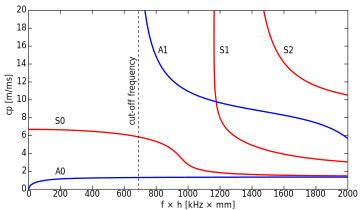
\includegraphics[width=1\linewidth]{Intro/dispersion}
	%	\end{center}
	\caption{Dispersion diagram for a 1 mm \ac{cfrp} plate (adopted from Dispersion Calculator~\cite{huber2021dispersion}). Red and blue solid curves represent symmetric and antisymmetric modes, respectively; a black dashed line indicates the cut-off frequency for higher modes.}
	\label{fig:dispersion}
\end{figure}
\begin{figure}
	%	\begin{center}
	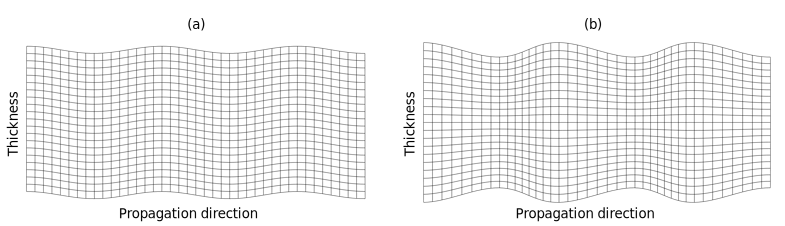
\includegraphics[width=1\linewidth]{Intro/mode_shape}
	%	\end{center}
	\caption{Mode shape of the \textbf{(a)} \ac{a0} and \textbf{(b)} \ac{s0} at 100 kHz for \(\phi=0^{\circ}\) in 2 mm composite plate (exported from Dispersion Calculator~\cite{huber2021dispersion}).}
	\label{fig:mode_shape}
\end{figure}

Detection schemes based on \acp{gw} exploit reflection, attenuation, and mode conversion when the propagating wave encounters a discontinuity in the structure \cite{alleyne1992interaction}.
Thus, this technique is efficient in detecting various types of defects, such as delamination \cite{sohn2011delamination,tian2015delamination}, adhesive disbonds \cite{rucka2018damage,balasubramaniam2021ultrasonic}, corrosion changes \cite{alleyne1995long,lowe1998defect}, cracks \cite{tua2004detection,lu2006crack,zima2020detection} and failures occurring in \acp{hsc} \cite{mustapha2011assessment, sikdar2016guided, sikdar2016ultrasonic,radzienski2016assessment, yu2019core}.
Many techniques based on \ac{gw} propagation have been developed for damage detection and localization.
A pitch-catch technique \cite{ihn2008pitch, sikdar2017structural} uses a pair of detached sensors, one excites, and the other receives a signal.
If the wave encounters a defect between the sensors, it will scatter, and the recorded signal will be distorted.
In the case of the pulse-echo technique \cite{guo1993interaction, kudela2008damage}, there is one sensor that excites the wave and, at the same time, registers possible echoes from the damage.
The damage localization can be determined if the wave speed is known and the time of flight is measured.
The radar principles were utilized in a phased array technique for plate inspection \cite{giurgiutiu2004embedded, ostachowicz2008elastic, kudela2018structural}.
The technique uses an array of transducers, each excited with an appropriate time offset, to focus all the waves at a single grid point of the area to be inspected.
A damage map is determined once the signals are obtained and processed for the entire grid.
Fink proposed a different approach, developing what he called a time-reversal mirror \cite{fink1992time}.
In this method, the wave propagates from one sensor to another, and then after time-reversal and dispersion compensation, the wave is re-emitted to the origin sensor.
The resulting signal will be a mirror image of the forcing signal only if the wave does not encounter damage along the way \cite{park2007time, eremin2016analytically}.

The \acp{pzt} can be used mutually as actuator-receiver pairs or as a single actuator with other types of devices, e.g. \ac{sldv}, \ac{fbg} sensors.
The \acp{pzt} generate high forces with broadband frequency, so methods based on \ac{gw} can detect various damage types of different sizes in a large inspected area.
Moreover, specific algorithms do not require a baseline model, and the method implementation is economically efficient.

\subsection{Electromechanical impedance methods}
\Ac{emi} spectroscopy is also an effective and powerful technique in \ac{shm} for real-time structural damage assessment \cite{park2003overview}.
The basis of this method is the influence of the mechanical impedance of the inspected host structure on the electrical impedance of the \ac{pzt} attached to the structure.
Assuming that the mechanical property of the sensor remains unchanged over the monitoring period, any changes in measurements of the electrical impedance can be considered a difference in the structure stiffness, which in turn can indicate that a defect has occurred.

Fundamentals of the \ac{emi} method were introduced by Liang et al. \cite{liang1994impedance}.
An analytical model of a \ac{pzt} actuator bonded to one end of a single degree of freedom mass-spring-damper system was presented in this pioneering work.
In the early papers, the authors adopted quasi-static sensor approximation until  Giurgiutiu and Zagrai \cite{giurgiutiu2000characterization} derived an expression where the sensor dynamic was incorporated.
The dynamics of a single \ac{pzt} with various boundary conditions (free, clamped and elastically constrained) and sensor attached to a beam were considered.
Further investigation was performed for the sensor bonded to the host structures was performed \cite{zagrai2001electro, giurgiutiu2005damage}.
Damage detection is realized by comparing the state of the structure with the reference state using overall statistical damage indices, e.g., the \ac{rmsd}, the \ac{mapd}, \ac{ccd} and \ac{pnn}.
Malinowski et al. \cite{malinowski2014characterisation, malinowski2015use} investigated the effects of \ac{emi} changes related to the state of the adhesive layer between two composite plates.
The technique has been used to evaluate weak bonds due to inadequate adhesive curing temperature, release agent and moisture contamination. This type of damage is not detectable using the method based on \ac{gw} propagation.
Experimental testing was conducted on weakened samples and compared with a reference.
The \ac{rms} of the conductance in the range of 3-5 MHz and the first thickness resonant frequency shift were considered for bond-line assessment.

An and Sohn \cite{an2012integrated} proposed a new damage detection technique that combines \ac{emi} and \ac{gw} advantages.
In the method, measured admittance characteristic is separated into two parts: active and passive.
\Ac{di} is a weighted sum of two indicators obtained from \ac{gw} signal and active admittance.
Because passive impedance is only sensitive to temperature variation, it is used for temperature compensation on both mentioned signals.
Instead of two \acp{di}, Sevillano et al. \cite{sevillano2016damage} proposed more integrated \ac{di} based on the electromechanical power dissipation of the \ac{pzt} sensor.

The \ac{emi} technique can detect damage, such as delamination or cracks, but is also sensitive to changes, such as weak bonds, which the \ac{gw} method is ineffective at detecting.
However, the \ac{emi} is a local method for the high frequency.
Giurgiutiu et al. \cite{giurgiutiu2001electro} obtained consistent results for crack detection in distances up to 40 mm in the frequency range 300-450 kHz. 
This method is also sensitive to environmental conditions such as temperature and humidity fluctuations\cite{bhalla2002practical} or loading variations \cite{lim2011impedance}.

%\subsection{Modal analysis techniques}
\input{Chapters/Intro/sec:chall2enges}

\section{Conclusions}
\label{sec:conclusionsIntro}

%% SECTION CONTENT ////////////////////////////////////////////////////////////////////////////////////
The Introduction briefly reviewed issues raised in the dissertation, i.e., composite materials, their construction and applications; definition of the \ac{shm} and application of the \ac{pzt} sensors in damage detection; and challenges in \ac{gw} propagation modelling for damage severity assessment in \acp{hsc}.

According to the literature review, a useful method for damage size assessment in \ac{hsc} is needed to enhance the safety of using composite structures.
In the dissertation, a novel approach for assessing the size of mechanical damage in a sandwich panel was proposed and developed using a \ac{gw} propagation technique.
This procedure involved actuation of elastic waves in the investigated structure, as well as their recording with the use of the \ac{pzt} setup.
The signals and a preliminary numerical analysis that defined a function of the impact of damage on wave propagation were used to estimate the defect severity.
The milestone of the dissertation was to prepare numerically effective model of \ac{gw} propagation in a sandwich panel.
The selection process of a suitable numerical modelling technique addressed the following issues:
\begin{itemize}
	\item flexibility to model the complex structure of the honeycomb core
	\item time efficiency due to the large number of \ac{dof} in the model
	\item possibility of parallel calculation on the \ac{gpu}.
\end{itemize}
% Set page numbering to arabic the first time we commence a chapter.
% This is required to get the page numbering correct.

% Note that the text in the [] brackets is the one that will
% appear in the table of contents, whilst the text in the {}
% brackets will appear in the main thesis.

%% CHAPTER HEADER /////////////////////////////////////////////////////////////////////////////////////
\chapter[Problem Statement]{Problem Statement}
\label{ch:problem}

%% CHAPTER INTRODUCTION ////////////////////////////////////////////////////////////////////////////////////

%% INCLUDE SECTIONS ////////////////////////////////////////////////////////////////////////////////////

Composite materials are used as structural components whose failure can have catastrophic consequences.
Although \ac{gw} based methods are promising for damage detection and localisation, they have not been widely reported to estimate the damage size.
A better understanding of the effect of damage on elastic wave propagation in \acp{hsc} will allow the development of robust and practical tools to evaluate this structure.

The principal aim of this dissertation is to propose a new approach for the severity of damage identification in the \ac{hsc} employing the \ac{pzt} sensors.
The essence of the method is the determination of damage influence function on characteristic parameters of the propagating waves in the structure.
This function is defined using a numerical model developed by the \ac{sem}.

Initially, the model is prepared for the healthy sample under various operating conditions such as ambient temperature.
Then parametric simulations for different damage scenarios are performed.
The \ac{madif} is determined based on the obtained results. 
This function determines the flaw size depending on the \acp{pzt} response.
Damage is considered to be a debonding between the core and the skin. 
The following objectives of the dissertation are:
\begin{itemize}
	\item Develop a robust and efficient numerical model of the propagating \ac{gw} in the \ac{hsc} with the temperature as an additional parameter.
	\item Validate the model experimentally.
	\item Determine the \ac{madif} to define damage influence on the propagating waves.
	\item Investigate the structure experimentally under various temperature conditions.
	\item Propose a framework of damage detection based on the \ac{madif}.
\end{itemize}

The objectives imposed lead to the thesis formulated as follows:
\begin{thesis*}  
	Model-assisted analysis of guided wave propagation is an effective tool for determining the damage severity in the honeycomb sandwich composites.
\label{thesis}
\end{thesis*}

Chapter~\ref{ch:method} presents the methods for developing a model-assisted damage severity assessment scheme.

Chapter~\ref{ch:sem} gives a theoretical background of the \ac{sem} for \ac{gw} propagation.
It includes derivation of mass, stiffness and damping matrices for 2D and 3D formulation; interface coupling algorithm; time integration scheme; and parallel implementation for GPU calculation.

Chapter~\ref{ch:simulation} provides the details of the sample configuration for the \ac{fcgm} and \ac{hcgm}.
The meshing process of individual components of \ac{shm} system, signal parameters and the damage model are presented.

The results of numerical simulations and experimental validation are presented in Chapter~\ref{ch:validation}.

The crucial part of the dissertation appears in Chapter \ref{ch:severity}. Based on the simulations performed and their experimental validation, the function of the damage size effect on the elastic wave propagation in \ac{hsc} is revealed, termed \ac{madif}.

Chapter~\ref{ch:tempEffects} includes the analysis of the GW propagation under variable temperature conditions.

The conclusion of the dissertation and final remarks are provided in Chapter~\ref{ch:summary}.


% Note that the text in the [] brackets is the one that will
% appear in the table of contents, whilst the text in the {}
% brackets will appear in the main thesis.

%% CHAPTER HEADER /////////////////////////////////////////////////////////////////////////////////////
\chapter[Concept of the Method]{Concept of the Method}
\label{ch:method}

%% CHAPTER INTRODUCTION ///////////////////////////////////////////////////////////////////////////////


%% INCLUDE SECTIONS ///////////////////////////////////////////////////////////////////////////////////

%% SECTION HEADER /////////////////////////////////////////////////////////////////////////////////////
\section{Modelling of the GW Propagation in the SCS}
\label{sec:modelling}

%% SECTION CONTENT ////////////////////////////////////////////////////////////////////////////////////

%% SUBSECTION HEADER //////////////////////////////////////////////////////////////////////////////////

The most common numerical modeling of the phenomenon of \ac{gw} in \acp{hsc} found in the literature is a calculation of the effective material properties of the honeycomb structure \cite{baid2015dispersion, mustapha2014leaky, qi2008ultrasonic,  shi1995derivation, sikdar2016guided}.
The properties are obtained from the analytical \cite{gibson1982mechanics, malek2015effective} or \ac{fem} \cite{catapano2014multi, chen2014analysis} analysis of the honeycomb \ac{rve}.
A comprehensive literature review on the homogenization of the honeycomb structure is presented in work of Ahmed \cite{ahmed2019homogenization}.
Replacing the core geometry with a homogeneous material has many advantages.
First and foremost, it simplifies the domain mesh so that convergence of the solution requires fewer working memory resources and increases the value of the critical time step.
In addition, the wave propagation velocity is determined by the simulation is in good agreement with the experiment.

However, this method cannot adequately represent the phenomenon of propagating wave interaction in honeycomb cells.
It causes the signal energy not to dissipate as it would in a real structure.
Song et al. \cite{song2009guided} analyzed the degree of energy dispersion function of core geometry and signal frequency.
A more accurate model will be achieved if the real geometry of the hexagonal cell is retained.
Ruzzenne et al. presented a parametric study to evaluate the dynamic behavior of the honeycomb and cellular structures through the \ac{fem} and the application of the theory of periodic structures \cite{ruzzene2003wave}.
Recently, the simulations of the wave propagation in the \acp{hsc} have been conducted with commercially available finite element code~\cite{ hosseini2013numerical,song2009guided, tian2015wavenumber, zhao2018wave}.

However, the finite element method \ac{pzt} modeling of \ac{gw} is inefficient as it requires a significant amount of memory and is time-consuming.
The computational efficiency of the \ac{fem} in case of \ac{gw} modeling in the \acp{hsc} can be improved by using the time-domain \ac{sem}.
The \ac{sem} was originally used for the numerical solution of the fluid flow in a channel by Patera \cite{patera1984spectral} but has also been successfully developed for elastic wave propagation~\cite{ostachowicz2011guided}.

Kudela proposed a model of the \ac{gw} in \acp{hsc} by the parallel implementation of the \ac{sem} \cite{kudela2016parallel}.
The wave excitation was realized by an external force applied at the point of the panel.
However, this model had a large number (1.5 million) of \acp{dof}, because cells of the core and skin plate were modeled by the \ac{3d} spectral elements; however, the simulation was limited to only one skin plate and a small dimension of the \ac{hsc} (\(179 \times 159 \) mm).

The above-mentioned drawbacks were motivation to propose a new model of the \ac{hsc}.
In the present paper, the skin plates, adhesive layers and each wall of the hexagonal core were modeled by the \ac{2d} spectral elements.
However, \ac{2d} elements have nodes only in a mid-plane; therefore, there is no direct linking between the two adjacent structures.
This connection was implemented by interface elements based on Lagrange multipliers \cite{ashwin2014formulation, fiborek20192d}.

Additionally, the signal was generated and recorded with \acp{pzt}.
A non-matching interface between the transducers and the skin was used to avoid a too complex mesh-likewise to the interfaces developed for the \ac{fem} \cite{flemisch2000elasto, flemisch2012non}. 
To the best of the authors’ knowledge, the present model has not been implemented yet for \acp{hsc}.

The parametric study conducted in the paper leads to the determination of a \ac{madif}, which defines the influence of the size of the composite defect on wave propagation.
In this case, the defect is assumed to be a disbond between the skin and the core.

%% SECTION HEADER /////////////////////////////////////////////////////////////////////////////////////
\section{Temperature effect on \acl{gw} propagation}
\label{sec:temp}
 
The high propagation velocities of \acp{gw} make a single measurement last up to 2~\unit{\micro\second}.
Compared to slow changes in ambient temperature (in seconds), the propagation phenomenon can be modelled for the stationary temperature field.
It was assumed that the temperature field can be obtained from temperature sensors at the moment of \ac{gw} excitation.
For simplicity, the model assumed a uniform temperature field.

According to \cite{lu2005methodology, kijanka2013gpu}, there are two main factors that influence how temperature affects the Lamb waves propagation. First, the thermal expansion of the plate causes the propagation path to be extended. As the coefficient of thermal expansion of the \ac{cfrp} is relatively low (-0.76 \unit[per-mode = symbol]{\micro\meter\per\kelvin} in longitudinal direction along the reinforcing fibres \cite{ahmed2012study}) it was neglected in the consideration.
The other is the temperature dependence of wave velocity due to the variation in material properties of the components.
In the presented models, only changes in the elastic modulus of \ac{hsc} components were considered, while the density changes were neglected.
The mechanical properties of the considered \ac{hsc} components at the reference temperature \(T_r=20\)\unit{\degreeCelsius} are included in Table~\ref{tab:properties}.
\begin{table}[H]
	\small
	\tabcolsep=0.5cm
	\centering
	\caption{\label{tab:properties}The mechanical properties of the materials at a reference temperature of +20\unit{\degreeCelsius}}
	\begin{tabular}{ccccc}\toprule
		\multirow{2}{*}{\textbf{Material}} & $\boldsymbol{E_{11}}$ & $\boldsymbol{E_{33}}$ & $\boldsymbol{\nu_{12}}$ & $\boldsymbol{\rho}$ \\ & \unit{\giga\pascal} & \unit{\giga\pascal} & -- & \unit[per-mode = symbol]{\kilogram\per\cubic\meter}\\
		\midrule
		Carbon & 275 & 27 & 0.2 & 1900\\
		Epoxy & 3.43 & 3.43 & 0.35 & 1250\\
		Aluminium & 69 & 69 & 0.33 & 2770\\
		Epoxy adhesive & 6 & 6 & 0.34 & 1200\\
		Cyanoacrylate glue & 3 & 3 & 0.34 & 1200\\	
		\ac{pzt} &  59 & 47 & 0.31 & 7850\\
		\bottomrule
	\end{tabular}
\end{table}
Young's modulus for the \ac{cfrp} skin was calculated accordingly to the methodology described in \cite{chamis1983simplified, salamone2009guided, sikdar2018effects}.
The significant changes in mechanical properties under temperature occur mainly in the polymer matrix, while the variation in the carbon fibre properties has a negligible effect on wave propagation.
In this model \cite{salamone2009guided, hopkins2012extreme}, the reduction of Young’s modulus of the resin \(E_m\) with temperature variation was assumed as
\begin{eqnarray}
	E_m(T)=F_m E_{m}(T_r),
	\label{eq:factor_temp}
	\nomtypeR[E]{$E$}{Young's modulus}{}{\unit{\giga\pascal}}%
	\nomtypeR[T]{$T$}{Temperature}{}{\unit{\degreeCelsius}}%
	\nomtypeR[Tr]{$T_r$}{Reference temperature}{}{\unit{\degreeCelsius}}%
\end{eqnarray}
where \(E_{m}(T_r)\) is Young’s modulus of the resin at the reference temperature, and \(F_m\) is the temperature degradation factor.
According to \cite{chamis1983simplified}, it equals
\begin{eqnarray}
F_m=\sqrt{\frac{T_{g0}-T}{T_{g0}-20}},
\nomtypeD[Fm]{$F_m$}{Temperature degradation factor}{}%
\nomtypeR[Tg0]{$T_{g0}$}{Glass transition temperature}{}{\unit{\degreeCelsius}}%
\label{eq:em_temp}
\end{eqnarray}
where \(T_{g0}\) is the glass transition temperature.
Effective temperature-dependent properties of the \ac{cfrp} skin are presented in Figure \ref{fig:cfrpEG}.
The values of Young's modulus along and across carbon fibres, \(E_{11}\) and \(E_{33}\), respectively are depicted in Figure \ref{fig:cfrpEG}(\textbf{a}), and shear modulus \(G_{12}\) and \(G_{23}\) in Figure \ref{fig:cfrpEG}(\textbf{b}).

\begin{figure}
	\begin{center}
		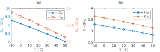
\includegraphics[width=0.95\textwidth]{Chapter_3/cfrpEG}
	\end{center}
	\caption{Temperature-dependent (\textbf{a}) Young's modulus (E\(_{11}\), E\(_{33}\)) and (\textbf{b}) shear modulus (G\(_{12}\), G\(_{23}\)) for the \acs{cfrp} skin}
	\label{fig:cfrpEG}
\end{figure}

Equation (\ref{eq:em_temp}) is also applicable to determine the elastic modulus of the adhesive layer.
The linear temperature dependence for aluminium given by Hopkins~et~al.~\cite{hopkins2012extreme} is defined as
\begin{eqnarray}
	E_a(T)=E_a(T_{r})+\num{4e7}(20-T).
	\label{eq:aluminium_temp}
\end{eqnarray}

Temperature-dependent properties of isotropic materials were determined according to the formulas and the fact that shear and Young's modulus are in relation as \(E=2G(1+\nu)\).
Young's modulus and shear modulus are presented in Figure \ref{fig:isoEG}(\textbf{a}) and Figure \ref{fig:isoEG}(\textbf{b}), respectively, for aluminium, adhesive layer and cyanoacrylate glue.
\begin{figure}[!tbh]
	\begin{center}
		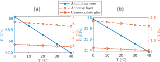
\includegraphics[width=0.95\textwidth]{Chapter_3/isoEG}
	\end{center}
	\caption{Temperature-dependent (\textbf{a}) Young's modulus (E) and (\textbf{b}) shear modulus (G) for isotropic materials used in the simulations}
	\label{fig:isoEG}
\end{figure}

Young's modulus and Poisson's ratio of the sensors were in the form proposed by Lanza et al. \cite{lanza2008temperature}:
\begin{eqnarray}
	\left(E_{11}\right)_{pzt}(T) & = & \left[\left(E_{11}\right)^{-1}_{pzt}(T_r) + \num{2.142857e-14}(20-T)\right]^{-1},\\
	\left(E_{33}\right)_{pzt}(T) & = & \left[\left(E_{33}\right)^{-1}_{pzt}(T_r) + \num{0.777142e-14}(20-T)\right]^{-1},\\
	\nu_{pzt}(T) & = & \nu_{pzt}(T_r) + \num{13e-3}(20-T).
	\label{eq:pzt_temp}
	\nomtypeD[nu]{\( \nu \)}{Poisson's ratio}{}
\end{eqnarray}

The piezo- and electromechanical properties were taken into account based on the
temperature characteristics provided by the manufacturer.
\begin{figure}[!tbh]
	\begin{center}
		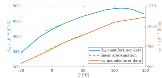
\includegraphics[width=0.95\textwidth]{Chapter_3/pzt_piezo_temp}
	\end{center}
	\caption{Temperature-dependent charge constant (\(d_{33}\)), and electric permittivity (\(\epsilon_{33}\)) of the \acs{pzt} provided by the manufacturer}
	\label{fig:pzt_temp}
\end{figure}
Due to the values provided by the manufacturer being in \(\pm10\%\) tolerance, the characteristics were approximated by the linear functions in the analysed range (see Figure \ref{fig:pzt_temp}) given in the form
\begin{eqnarray}
	\boldsymbol{d}(T) & = & \boldsymbol{d}(T_r) + \left[
	\begin{array}{cccccc}
		0 & 0 & 0 & 0 & 0 & 0\\
		0 & 0 & 0 & 0 & 0 & 0\\
		0.71 & 0.71 & -1.74 & 0 & 0 & 0
	\end{array}\right]\,(20-T) \times10^{-12},\\
	\boldsymbol{\epsilon}^S(T) & = & \boldsymbol{\epsilon}^S(T_r) - \left[
	\begin{array}{ccc}
		3.61 & 0 & 0\\
		0 & 3.61 & 0\\
		0 & 0 & 3.28
	\end{array}\right]\,(20-T) \times10^{-11},\\
	\textbf{e}(T) & = & \boldsymbol{d}(T)\,\textbf{c}_{PZT}(T),
	\label{eq:piezo_temp}
	\nomtypeG{\(\epsilon\)}{Electric permittivity}{}{\unit[per-mode = symbol]
		{\farad\per\metre}}%
	\nomtypeR[d]{\(d\)}{Charge constant}{}{\unit[per-mode = symbol]
		{\coulomb\per\newton}}%
	\nomtypeR[e]{\(e\)}{Piezoelectric coupling coefficient}{}{\unit[per-mode = symbol]
		{\coulomb\per\square\metre}}%
\end{eqnarray}
were \(\boldsymbol{\epsilon}^S\) is the electric permittivity measured at zero strain, \(\boldsymbol{d}\) is the charge constant matrix, \(\boldsymbol{e}\) is the piezoelectric coupling coefficients matrix and \(\boldsymbol{c}_{PZT}\) is the elastic stiffness matrix. 
The manufacturer provided the following piezo constant matrices for reference temperature:
\begin{eqnarray}
	\boldsymbol{d}(T_r) & = & \left[
	\begin{array}{cccccc}
	0 & 0 & 0 & 0 & 669 & 0\\
	0 & 0 & 0 & 669 & 0 & 0\\
	-208 & -208 & 443 & 0 & 0 & 0
	\end{array}\right] \times10^{-12}\ \unit[per-mode = symbol]{\coulomb\per\newton},\\
	\boldsymbol{\epsilon}^S(T_r) & = & \left[
	\begin{array}{ccc}
	802 & 0 & 0\\
	0 & 802 & 0\\
	0 & 0 & 729
\end{array}\right] \times10^{-11}\ \unit[per-mode = symbol]{\farad\per\meter}.
\end{eqnarray}

\begin{figure}[!tbh]
	\begin{center}
		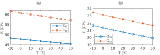
\includegraphics[width=0.95\textwidth]{Chapter_3/pztEG}
	\end{center}
	\caption{Temperature-dependent \textbf{(a)} Young's modulus (E\(_{11}\), E\(_{33}\)) and \textbf{(b)} shear modulus (G\(_{12}\), G\(_{23}\)) for the \acs{pzt}}
	\label{fig:pztEG}
\end{figure}

Temperature-dependent mechanical coefficients for the \ac{pzt} are shown in Figure~\ref{fig:pztEG}(\textbf{a}) for Young's modulus and in Figure~\ref{fig:pztEG}(\textbf{b}) for shear modulus.
For~piezoelectric coupling coefficients (\(e_{31},\ e_{15},\ e_{33}\)) and electric permittivity (\(\epsilon^S_{11},\  \epsilon^S_{33}\)), temperature-dependent characteristics are shown in Figures~\ref{fig:pztEEps}(\textbf{a}) and ~\ref{fig:pztEEps}(\textbf{b}), respectively.


\begin{figure}[!tbh]
	\begin{center}
		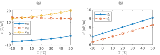
\includegraphics[width=0.95\textwidth]{Chapter_3/pztEEps}
	\end{center}
	\caption{Temperature-dependent (\textbf{a}) piezoelectric coupling coefficients (e\(_{31}\), e\(_{15}\), e\(_{33}\)) and (\textbf{b}) electric permittivity (\(\boldsymbol{\epsilon}^S_{11}\), \(\boldsymbol{\epsilon}^S_{33}\)) for the \acs{pzt}}
	\label{fig:pztEEps}
\end{figure}
\nomtypeG[\(\rho\)]{\( \rho \)}{Mass density}{}{\unit[per-mode = symbol]
	{\kilogram\per\cubic\metre}}

%%% SECTION HEADER /////////////////////////////////////////////////////////////////////////////////////
\section{Model-Assisted Damage Identification Function}
\label{sec:madif}

%% SECTION CONTENT ////////////////////////////////////////////////////////////////////////////////////
he severity of damage was estimated based on the function determined with the numerical simulation.
A simple flowchart given in Figure~\ref{fig:Flowchart} represents a process for the sample assessment.
When the structure model is developed, several computer simulations for various damage sizes must be conducted to determine the \ac{madif}.
%\begin{figure}[H]
%	%	\begin{center}
%	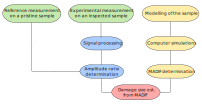
\includegraphics[width=1\linewidth]{Chapter_7/flowchart}
%	%	\end{center}
%	\caption{A flowchart representing the process for damage size estimation.}
%	\label{fig:Flowchart}
%\end{figure}
The \ac{madif} indicates the damage size according to measured damage index \(I\) normalized by the value obtained for the pristine sample \(I^{ref}\).
In the paper, two types of damage index \(I\) are considered: the energy \(I_{eng}\) and the maximum value of the half-width of the first package arrived in the sensor \(I_{amp}\), and these are defined as:
\begin{eqnarray}
	I_{eng}(\Phi_D)=\sum_{t=0}^{T} \left (\Psi_g(t,\Phi_D)\right )^2,\quad I_{eng}^{ref}=\sum_{t=0}^{T} \left (\Psi_g(t,0)\right )^2,\\
	I_{amp}(\Phi_D)=\mathrm{max}\left ( \Psi_g(t,\Phi_D)\right ),\quad I_{amp}^{ref}=\mathrm{max}\left ( \Psi_g(t,0)\right ),
	\label{eq:I_amp}
\end{eqnarray}
where \textit{T} is a period of the signal.
\(\Psi_g(t,\Phi_D)\) is for the damaged case scenario, whereas \(\Psi_g(t,0)\) is for the pristine sample and it is realized in the same way by windowing the full-length signals of the sensor \(\Psi(t)\) with a flattened Gaussian window \emph{g(t)} as follows:
\begin{eqnarray}
	\Psi_g(t)=\Psi(t)g(t)= \Psi(t)\mathrm{exp}\left(-\left(\frac{t-t_0}{0.6005612w_g}\right) ^{12}\right),
	\label{eq:psi_g}
\end{eqnarray}
where \(t_0\) is the center and \(w_g=0.5N_c/f_c\) is a half-width of the window.
Windowing the signals ensures obtaining the signals without any reflections from the boundaries.
The determination of \(\Psi_g\) is pictured in Figure~\ref{fig:window_madif}a.

\begin{figure}[H]
	%	\begin{center}
	\includegraphics[width=1\linewidth]{Chapter_7/window_madif_03}
	%	\end{center}
	\caption{(\textbf{a}) The %MDPI: The hyphen in the picture should be changed to minus sign, e.g., ``-0.5'' to ``$-$0.5'', please change. Please check all like this in all figures. 
		sensor signal \(\Psi(t)\) windowed by a flattened Gaussian window \(g(t)\) and (\textbf{b}) the damage size estimation from the \ac{madif}.}
	\label{fig:window_madif}
\end{figure}
In the time domain, an equivalent numerical signal to the signal registered by the \ac{pzt} acquisition instrument is calculated as an average value of the electrical potential of the electrode surface
\begin{eqnarray}
	\Psi^{n}(t) = \frac{\int_{\Gamma_e}\phi\mathrm{d}\Gamma}{\Gamma_e},
	\label{eq:psi}
\end{eqnarray}
where \(n=1\) and \(n=2\) correspond to the homogenized and presented model, respectively.

The \ac{madif} is achieved by approximating the inverse of the computed damage index that best matches the experimental one.
Finally, the damage size \(\Phi_D\) is obtained from the \ac{madif} curve for measuring the normalized value of \(I/I^{ref}\) as it is presented in Figure~\ref{fig:window_madif}b.
%% SECTION HEADER /////////////////////////////////////////////////////////////////////////////////////
\section{Conclusions}
\label{sec:conclusionsMethod}

%% SECTION CONTENT ////////////////////////////////////////////////////////////////////////////////////




% Note that the text in the [] brackets is the one that will
% appear in the table of contents, whilst the text in the {}
% brackets will appear in the main thesis.

%% CHAPTER HEADER /////////////////////////////////////////////////////////////////////////////////////
\chapter[The Time-Domain Spectral Element Method Formulation]{The Time-Domain Spectral Element Method Formulation}
\label{ch:sem}

%% CHAPTER INTRODUCTION ///////////////////////////////////////////////////////////////////////////////

%% INCLUDE SECTIONS ///////////////////////////////////////////////////////////////////////////////////

%% SECTION HEADER /////////////////////////////////////////////////////////////////////////////////////
\section{The Spectral Element Method}
\label{sec:sem}

%% SECTION CONTENT ////////////////////////////////////////////////////////////////////////////////////

The general concept of the \ac{sem} is based on the idea of the \ac{fem}.
The similarity of both methods lies in the fact that the modeled domain is divided into non-overlapping finite elements, and external forces and arbitrary boundary conditions are imposed in the particular nodes.
The main difference between those methods is a choice of the shape function \( N=N(\xi )\), which is interpolated by a Lagrange polynomial that passes through the element nodes. The nodes are localized on the endpoint of an interval, \(\xi\in[-1,1]\), and the roots of the first derivative of Legendre polynomial P of degree \(p-1\):
\begin{eqnarray}
	(1-\xi^2)P'_{p-1}(\xi)=0.
	\label{eq:nodes}
\end{eqnarray}

The approximation of an integral over the elements is achieved according to \ac{gll} rule at points coinciding with the element nodes, 
and the weights \(w=w(\xi)\) calculated as:
\begin{eqnarray}
	{w(\xi)} = \frac{2}{p(p-1)(P_{p-1}(\xi))^2}.
	\label{eq:weights}
\end{eqnarray}

This approach guarantees a diagonal mass matrix.
The shape functions and the weights for \ac{2d} or \ac{3d} elements are obtained by the Kronecker product of vectors of individual axes, denoted by \(\otimes\) as follows:
\begin{eqnarray}
	N(\xi,\eta) = N(\xi)\otimes N(\eta), & N(\xi,\eta,\zeta) = N(\xi)\otimes N(\eta)\otimes N(\zeta), \nonumber\\
	w(\xi,\eta) = w(\xi)\otimes w(\eta), & w(\xi,\eta,\zeta) = w(\xi)\otimes w(\eta)\otimes w(\zeta).
	\label{eq:3Dshape_weights}
\end{eqnarray}

The elementary equations of motion is defined as:
\begin{eqnarray}
	\label{eq:motion}
	\textbf{M} \ddot{\textbf{d}} + \textbf{D} \dot{\textbf{d}} + \textbf{K} \textbf{d} = \textbf{F}_{ext}
\end{eqnarray}
where \textbf{d} is the displacement vector; \textbf{M}, \textbf{D}, \textbf{K} are structural mass, damping and stiffness matrices, respectively; \textbf{F}$_{ext}$ is the external forces vector; \((\dot{\ })=\frac{\partial}{\partial t}\). Construction of the \textbf{M}, \textbf{D}, \textbf{K} matrices is similar to the classical approach in \ac{fem}.

The convergence of the equation~(\ref{eq:motion}) in the \ac{sem} is already achieved for six nodes per wavelength, while at least fifteen nodes are needed in case of linear elements in classic \ac{fem}~\cite{wee2017simulating}. Moreover, the mass matrix is diagonal when the \ac{gll} approach is used.


%% SECTION HEADER /////////////////////////////////////////////////////////////////////////////////////
\section{2D Spectral Modelling}
\label{sec:2Dmodel}

%% SECTION CONTENT ////////////////////////////////////////////////////////////////////////////////////

According to the first-order shear deformation theory~\cite{reissner1945effect, mindlin1951influence}, the displacement field is expressed as:
\begin{eqnarray}
	\left \{ \begin{array}{c}
		\textbf{u}^e(\xi,\eta) \\
		\textbf{v}^e(\xi,\eta) \\
		\textbf{w}^e(\xi,\eta)
	\end{array} \right\} = 
	\left \{ \begin{array}{c}
		\textbf{u}_0^e(\xi,\eta) + z\boldsymbol{\varphi}_x^e(\xi,\eta)\\
		\textbf{v}_0^e(\xi,\eta) + z\boldsymbol{\varphi}_y^e(\xi,\eta)\\
		\textbf{w}_0^e(\xi,\eta) \\
	\end{array} \right\},
\end{eqnarray}
where \(\textbf{u}_0^e\), \(\textbf{v}_0^e\) and \(\textbf{w}_0^e\) are nodal displacements, \(\boldsymbol{\varphi}_x^e\), \(\boldsymbol{\varphi}_y^e\) are the rotations of the normal to the mid-plane with respect to the axes \textit{x} and \textit{y}, respectively.
\begin{eqnarray}
	\left \{\begin{array}{c}
		\textbf{u}_0^e(\xi,\eta) \\
		\textbf{v}_0^e(\xi,\eta) \\
		\textbf{w}_0^e(\xi,\eta) \\
		\boldsymbol{\varphi}_x^e(\xi,\eta) \\
		\boldsymbol{\varphi}_y^e(\xi,\eta)
	\end{array} \right\}
	= \textbf{N}^e(\xi,\eta)\widehat{\textbf{d}}^e
	= \sum_{n=1}^q\sum_{m=1}^p\textbf{N}_m^e(\xi)\textbf{N}_n^e(\eta)
	\left \{ \begin{array}{c}
		\widehat{\textbf{u}}_0^e \\
		\widehat{\textbf{v}}_0^e \\
		\widehat{\textbf{w}}_0^e \\
		\widehat{\boldsymbol{\varphi}}_x^e \\
		\widehat{\boldsymbol{\varphi}}_y^e
	\end{array} \right \}.
\end{eqnarray}

The nodal bending strain--displacement relations are given in the form:
\begin{eqnarray}
	\boldsymbol{\epsilon}_b^e =
	\textbf{B}_b^e\widehat{\textbf{d}}^e = 
	\left [
	\begin{array}{ccccc}
		\frac{\partial N^e}{\partial x} & 0 & 0 & 0 & 0\\
		0 & \frac{\partial N^e}{\partial y} & 0 & 0 & 0\\
		\frac{\partial N^e}{\partial y} & \frac{\partial N^e}{\partial x} & 0 & 0 & 0\\
		0 & 0 & 0 & -\frac{\partial N^e}{\partial x} & 0\\
		0 & 0 & 0 & 0 & -\frac{\partial N^e}{\partial y}\\
		0 & 0 & 0 & -\frac{\partial N^e}{\partial y} & -\frac{\partial N^e}{\partial x}
	\end{array} \right]
	\left \{ \begin{array}{c}
		\widehat{\textbf{u}}_0^e \\
		\widehat{\textbf{v}}_0^e \\
		\widehat{\textbf{w}}_0^e \\
		\widehat{\boldsymbol{\varphi}}_x^e \\
		\widehat{\boldsymbol{\varphi}}_y^e
	\end{array} \right\}.
\end{eqnarray}

The nodal shear strain--displacement relations are given in the form:
\begin{eqnarray}
	\boldsymbol{\epsilon}_s^e =
	\textbf{B}_s^e\widehat{\textbf{d}}^e = 
	\left [
	\begin{array}{ccccc}
		0 & 0 & \frac{\partial N^e}{\partial y} & -1 & 0\\
		0 & 0 & \frac{\partial N^e}{\partial y} & 0 & -1
	\end{array} \right]
	\left \{ \begin{array}{c}
		\widehat{\textbf{u}}_0^e \\
		\widehat{\textbf{v}}_0^e \\
		\widehat{\textbf{w}}_0^e \\
		\boldsymbol{\varphi}_x^e \\
		\boldsymbol{\varphi}_y^e
	\end{array} \right\}.
\end{eqnarray}
%% SECTION HEADER /////////////////////////////////////////////////////////////////////////////////////
\section{\acs{3d} spectral element}
\label{sec:3Dmodel}

%% SECTION CONTENT ////////////////////////////////////////////////////////////////////////////////////
The displacement vector of the element based on \ac{3d} elasticity of solids is composed of three translational displacements defined as:
\begin{eqnarray}
	\begin{split}
	\left \{ \begin{array}{c}
		\textbf{u}^e(\xi,\eta,\zeta) \\
		\textbf{v}^e(\xi,\eta,\zeta) \\
		\textbf{w}^e(\xi,\eta,\zeta)
	\end{array} \right\}
	& = \textbf{N}^e(\xi,\eta, \zeta)\widehat{\textbf{d}}^e\\
	& = \sum_{l=1}^r\sum_{n=1}^q\sum_{m=1}^p\textbf{N}_m^e(\xi)\textbf{N}_n^e(\eta)\textbf{N}_l^e(\zeta)
	\left \{ \begin{array}{c}
		\widehat{\textbf{u}}^e(\xi_m,\eta_n,\zeta_l) \\
		\widehat{\textbf{v}}^e(\xi_m,\eta_n,\zeta_l) \\
		\widehat{\textbf{w}}^e(\xi_m,\eta_n,\zeta_l)
	\end{array} \right\},
	\label{eq:3D_displ}
	\end{split}
\end{eqnarray}
where \(\widehat{\textbf{u}}^e\), \(\widehat{\textbf{v}}^e\) and 
\(\widehat{\textbf{w}}^e\) are displacements of the element nodes in \(\xi,\eta\) and \(\zeta\) direction.

The nodal strain--displacement relations are given as \cite{kudela20093d}:
\begin{eqnarray}
	\boldsymbol{\varepsilon}^e=\textbf{B}^e\widehat{\textbf{d}}^e=
	\left [
	\begin{array}{ccc}
		\frac{\partial N^e}{\partial x} & 0 & 0\\
		0 & \frac{\partial N^e}{\partial y} & 0\\
		0 & 0 & \frac{\partial N^e}{\partial z}\\
		0 & \frac{\partial N^e}{\partial z} & \frac{\partial N^e}{\partial y}\\
		\frac{\partial N^e}{\partial z} & 0 & \frac{\partial N^e}{\partial x}\\
		\frac{\partial N^e}{\partial y} & \frac{\partial N^e}{\partial x} & 0
	\end{array} \right]
	\left \{ \begin{array}{c}
		\widehat{\textbf{u}}^e \\
		\widehat{\textbf{v}}^e \\
		\widehat{\textbf{w}}^e
	\end{array} \right\}.
\end{eqnarray}
The formulae of the structural matrices for \ac{3d} elements are:
\begin{eqnarray}
	\textbf{M}_{dd}^e & = & \int_{V^e}\textbf{N}^{\mathrm{T}}\rho \textbf{N} \diff V^e,\\
	\textbf{K}_{dd}^e & = & \int_{V^e}{\textbf{B}_d^e}^{\mathrm{T}}\textbf{c}\textbf{B}_d^e \diff V^e,
\end{eqnarray}
\nomtypeR[Ve]{$V^e$}{Element volume}{-}{\unit{\cubic\meter}}%
where \textbf{c} is the elasticity tensor, \(\rho\) is mass density, and \(V_e\) is the element volume.
%% SECTION HEADER /////////////////////////////////////////////////////////////////////////////////////
\section{Piezoelectric Transducers Modelling}
\label{sec:PZTmodel}

%% SECTION CONTENT ////////////////////////////////////////////////////////////////////////////////////
The electromechanical coupling is governed by the linear constitutive equation of piezoelectric material according to~\cite{giurgiutiu2009micromechatronics, rekatsinas2017cubic}, and this is defined as:
\begin{eqnarray}
	\left [ 
	\begin {array}{c}
	\boldsymbol{\sigma}\\
	\textbf{D}
\end{array}\right ]=
\left [ 
\begin{array}{cc}
	\textbf{c}^E & -\textbf{e}^T \\
	\textbf{e} & \epsilon^S 
\end{array} \right ]
\left[ 
\begin{array}{c}
	\textbf{S}\\
	\textbf{E} 
\end{array} \right ],
\label{eq:elecmechcoupling}
\end{eqnarray}
where \(\boldsymbol{\sigma}\) and \(\textbf{S}\) are the stress and strain components, respectively, \(\textbf{c}^E\) is the stiffness coefficient matrix measured at zero electric field, \textbf{e} is the piezoelectric coupling tensor,  \(\boldsymbol{\epsilon}^S\) is the electric permittivity, and \textbf{E} and \textbf{D} are the electric field and electric displacement measured at zero strain.
The superscript T denotes a transpose matrix.
The electric field is defined as:
\begin{eqnarray}
\textbf{E}^e=-\textbf{B}_\phi^e \widehat{\boldsymbol{\phi}}^e = \left[ \begin{array}{c}
	\frac{\partial N^e}{\partial \xi}\\
	\frac{\partial N^e}{\partial \eta}\\
	\frac{\partial N^e}{\partial \zeta}
\end{array} \right] \widehat{\boldsymbol{\phi}}^e,
\end{eqnarray}
where \(\widehat{\boldsymbol{\phi}}^e\) is a nodal voltage of the transducer. The \ac{sem} formulation of the governing equation (\ref{eq:elecmechcoupling}) is defined as:
\begin{eqnarray}
	\left [\begin{array}{cc}
		\textbf{M}_{dd} & \textbf{0}\\
		\textbf{0} & \textbf{0}
	\end{array}\right]
	\left \{\begin{array}{c}
		\widehat{\ddot{\textbf{d}}} \\
		\textbf{0}
	\end{array}\right \} +
	\left [\begin{array}{cc}
		\textbf{K}_{dd} & \textbf{K}_{d \phi}\\
		\textbf{K}_{d \phi}^T & \textbf{K}_{\phi \phi}
	\end{array}\right]
	\left \{\begin{array}{c}
		\widehat{\textbf{d}} \\
		\widehat{\boldsymbol{\phi}}
	\end{array}\right \}  = 
	\left \{\begin{array}{c}
		\textbf{0}\\
		\widehat{\textbf{Q}}
	\end{array}\right \},
	\label{eq:pzt_sem}
\end{eqnarray}
where \(widehat{\textbf{Q}}\) is the nodal charge vector.
The mass and stiffness matrices are defined according to \ac{3d} model from section \ref{sec:3Dmodel}.
The piezoelectric coupling matrix \(\textbf{K}_{\phi \phi}^e\) and the dielectric permittivity matrix \(\textbf{K}_{d \phi}^e\) are defined as:
\begin{eqnarray}
	\textbf{K}_{d\phi}^e & = & \int_{V_e}{\textbf{B}_d^e}^T\textbf{e}^T \textbf{B}_{\phi}^e \diff V_e,\\
	\textbf{K}_{\phi \phi}^e & = & -\int_{V_e}{\textbf{B}_{\phi}^e}^T 
	{\textbf{\(\epsilon\)}^S}^T \textbf{B}_{\phi}^e \diff V_e.
\end{eqnarray}

If a vector \(\textbf{b}\) contains list of consecutive boundary nodes (electrodes) and a vector \(\textbf{a}\) contains lists of consecutive active nodes (remains nodes) of the \ac{pzt}, the electrical potential vector and the charge vector can be rewritten as:
\begin{eqnarray}
	\widehat{\boldsymbol{\phi}} & = & \left \{\begin{array}{cc}
		\widehat{\boldsymbol{\phi}}(\textbf{b}) &
		\widehat{\boldsymbol{\phi}}(\textbf{a})
	\end{array}\right \}^T,\\
	\widehat{\textbf{Q}} & = & \left \{\begin{array}{cc}
		\widehat{\textbf{Q}}(\textbf{b}) & \textbf{0}
	\end{array}\right \}^T.
	\label{eq:phi_Q}
\end{eqnarray}
Then, piezoelectric part of Equation~(\ref{eq:pzt_sem}) is expressed as:
\begin{eqnarray}
	\left [\begin{array}{cc}
		\textbf{K}_{d \phi}(:,\textbf{b}) &
		\textbf{K}_{d \phi}(:,\textbf{a})
	\end{array}\right]^T
	\widehat{\textbf{d}} +
	\left [\begin{array}{cc}
		\textbf{K}_{\phi \phi}(\textbf{b},\textbf{b}) & \textbf{K}_{\phi \phi}(\textbf{b},\textbf{a})\\
		\textbf{K}_{\phi \phi}(\textbf{a},\textbf{b}) & \textbf{K}_{\phi \phi}(\textbf{a},\textbf{a})
	\end{array}\right]
	\left \{\begin{array}{c}
		\widehat{\boldsymbol{\phi}}(\textbf{b}) \\
		\widehat{\boldsymbol{\phi}}(\textbf{a})
	\end{array}\right \} = 
	\left \{\begin{array}{c}
		\widehat{\textbf{Q}}(\textbf{b}) \\
		\textbf{0}
	\end{array}\right \},
	\label{eq:pztboundary}
\end{eqnarray}
where the notation \(\textbf{K}(\textbf{r},\textbf{c})\) uses vectors \(\textbf{r}\) and \(\textbf{c}\) to extract rows and columns from the matrix \(\textbf{K}\), respectively, and \((:)\) means all rows or columns of \(\textbf{K}\).
The electrical potential of the free nodes can be extracted from Equation~(\ref{eq:pztboundary}):
\begin{eqnarray}
	\widehat{\boldsymbol{\phi}}(\textbf{a}) = -\textbf{K}_{\phi\phi}^{-1}(\textbf{a},\textbf{a})\left[\textbf{K}_{\phi d}(\textbf{a},:) \widehat{\textbf{d}} + \textbf{K}_{\phi\phi}(\textbf{a},\textbf{b})\widehat{\boldsymbol{\phi}}(\textbf{b}) \right].
	\label{eq:freePotetial}
\end{eqnarray}
If the \ac{pzt} acts as an actuator, the electrical potential of the electrode nodes has the values of the applied signal.
As one of the electrodes is grounded, the potential is zero.
Therefore, the potential vector can be written as:
\begin{eqnarray}
	\widehat{\boldsymbol{\phi}}(\textbf{b}) = \left \{\begin{array}{cc}
		\widehat{\boldsymbol{\phi}}(\textbf{b}_v) &
		\widehat{\boldsymbol{\phi}}(\textbf{b}_g)
	\end{array}\right \}^T=\left \{\begin{array}{cc}
	\textbf{V}(t) & \textbf{0}
	\end{array}\right \}^T,
	\label{eq:phi_V}
\end{eqnarray}
where \(\textbf{b}_v\) is a list of nodes of the applied electrode and \(\textbf{b}_g\) is a list of nodes of the grounded electrode.
Substituting Equation (\ref{eq:phi_V}) into Equations (\ref{eq:freePotetial}) and (\ref{eq:pztboundary}) induced stiffness of the actuator is obtained:
\begin{eqnarray}
	\textbf{K}_{a}=-\textbf{K}_{d\phi}(:,\textbf{a})\,\textbf{K}_{\phi \phi}^{-1}(\textbf{a},\textbf{a})\,\textbf{K}_{\phi \phi} (\textbf{a},\textbf{b}).
\end{eqnarray}
Hence, the equivalent mechanical force vector of the applied voltage of the piezoelectric actuator equals:
\begin{eqnarray}
	\widehat{\textbf{f}}_{act}=-\textbf{K}_{a}\,\widehat{\boldsymbol{\phi}}(\textbf{b}).
	\label{eq:f_act}
\end{eqnarray}

In the case of the open circuit sensor one electrode is grounded so the electric potential of the free nodes becomes as:
\begin{eqnarray}
	\widehat{\boldsymbol{\phi}}(\textbf{a}) = -\textbf{K}_{\phi\phi}^{-1}(\textbf{a},\textbf{a})\,\textbf{K}_{\phi d}(\textbf{a},:)\,\widehat{\textbf{d}}.
	\label{eq:sensorPotetial}
\end{eqnarray}
The induced stiffness of the sensor can be written as:
\begin{eqnarray} \textbf{K}_s=\textbf{K}_{d \phi}(:,\textbf{a})\,\textbf{K}_{\phi \phi}^{-1} (\textbf{a},\textbf{a})\,\textbf{K}_{\phi d}(\textbf{a},:).
\end{eqnarray}
To obtain the sensor response nodal electric potential must be integrated over the electrode surface as follow:
\begin{eqnarray}
	\boldsymbol{\phi}(t) = \int_{\Omega_s}\widehat{\phi} \diff\Omega_s.
	\label{eq:sensorResponse}
\end{eqnarray}
%% SECTION HEADER /////////////////////////////////////////////////////////////////////////////////////
\section{Structural damping}
\label{sec:damping}

%% SECTION CONTENT ////////////////////////////////////////////////////////////////////////////////////
Propagating waves in the structure attenuate due to many factors, including geometric spreading, material damping, and dissipation into the adjacent domain.
This study adopted the Rayleigh damping model for the \ac{cfrp} skin and adhesive layer, while the damping for the aluminium core and \ac{pzt} was neglected.
Rayleigh damping model is defined as \cite{wandowski2017guided}:
\begin{eqnarray}
	\textbf{D}_{dd}^e = \alpha_M \textbf{M}_{dd}^e + \beta_K \textbf{K}_{dd}^e,
	\label{eq:damping}
\end{eqnarray}
where \(\alpha_M\) and \(\beta_K\) are the mass- and stiffness- proportionality coefficients.
In presented model, \(\beta_K\) was assumed equal to zero to ensure that matrix \(\textbf{D}_{dd}\) remains diagonal \cite{schulte2011simulation, wandowski2017guided}.
This assumption gives a good approximation when considering a single mode and a specific frequency. 
Ramadas showed slight differences in Lamb wave attenuation by analysing three models, i.e. mass-, stiffness-proportional and the sum of both \cite{ramadas2011modelling}.
However, the mass-proportional model is computationally incomparable to the other models due to the diagonal damping matrix.
%% SECTION HEADER /////////////////////////////////////////////////////////////////////////////////////
\section{Displacements coupling at the interface of substructures}
\label{sec:interface}

%% SECTION CONTENT ////////////////////////////////////////////////////////////////////////////////////

The present model of the sandwich panel consists of \ac{2d} and \ac{3d} elements. 
Moreover, there are non-matching grids between two adjacent substructures. 
These involve connecting them by imposing the compatibility of the displacements at the interface, see Fig.~\ref{fig:interface}.
This type of connection is implemented through the interface elements based on Lagrange multipliers, which are interpreted as forces responsible for determining the appropriate displacements of nodes.
The coupling can be expressed as:
\begin{eqnarray}
	\left\{\begin{array}{c}
		\textbf{u}\\
		\textbf{v}\\
		\textbf{w}
	\end{array}\right\}_{s_{i1}}^{\Gamma^i}-
	\left\{\begin{array}{c}
		\textbf{u}\\
		\textbf{v}\\
		\textbf{w}
	\end{array}\right\}_{s_{i2}}^{\Gamma^i}=
	\left\{\begin{array}{c}
		\textbf{0}\\
		\textbf{0}\\
		\textbf{0}
	\end{array}\right\},
	\label{eq:coupling}
\end{eqnarray}
\begin{figure}
	\begin{center}
		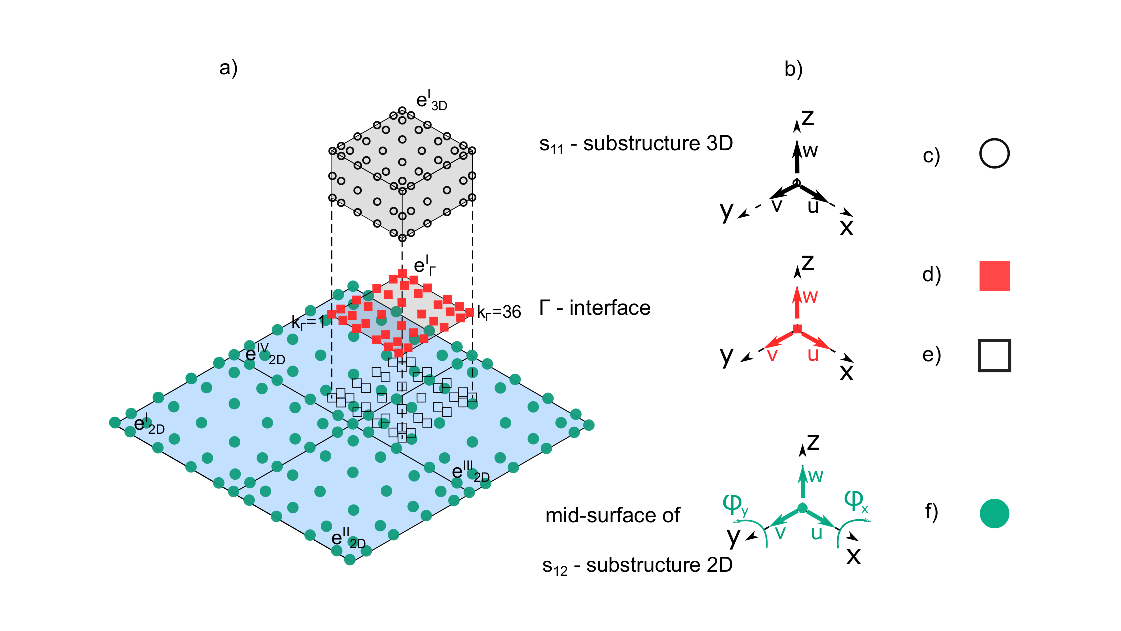
\includegraphics[width=0.95\textwidth]{Chapter_4/interface_2D3D}
	\end{center}
	\caption{Non-matching interface setup: a) interface coupling, b) degrees-of-freedom of the interface and the substructures.}
	\label{fig:interface}
\end{figure}
where \(s_{i1}\) and \(s_{i2}\) are substructures connected by the interface \(\Gamma^i\). For the whole structure, the Eq.~(\ref{eq:coupling}) can be written in the matrix form:
\begin{eqnarray}
	\textbf{G}\textbf{d}=\textbf{0},
	\label{eq:cond_disp}
\end{eqnarray}
where \textbf{G} is the coupling matrix which contains the equations to interpolate the substructures displacements at the interfaces, and \(\textbf{d}\) is a global displacement field for \(nS\) number of substructures, composed as:
\begin{eqnarray}
	\textbf{d} = \left\{\begin{array}{cccc}
		\textbf{d}_1, & \textbf{d}_2, &\ldots, & \textbf{d}_{nS}
	\end{array}\right\}^T.
	\label{eq:displacements}
\end{eqnarray}

General formulation of the matrix \textbf{G} is presented in Algorithm \ref{alg:G_matrix}.

\begin{algorithm}[H]
	\SetAlgoLined
	\KwResult{coupling matrix \textbf{G}}
	\For{i = 1 \KwTo 2}{
		create \(n^{\Gamma}\times n^{s_i}\) null matrix 
		\(\mathbf{G}_i\),\\
		\For{j = 1 \KwTo \(n^{\Gamma}\)} {
			find \(ownerElement^j_i\) in the structure \(s_i\) 
			containing interface node \(j\) with global coordinates vector: 
			\(X_p=(x^j_p,y^j_p)\)\;
			assign vector \(X_e=(x_e,y_e)\) of coordinates of all nodes in 
			\(ownerElement^j_i\)\;
			assign initial coordinates 
			\(X_{\kappa}=(x^j_{\kappa},y^j_{\kappa})\) to the nearest node in
			\(ownerElement^j_i\) to node \(j\)\;
			transform global coordinates \(X_{\kappa}\) to a local coordinate system \(\xi_{\kappa}=\xi(X_{\kappa});\quad 
			\eta_{\kappa}=\eta(X_{\kappa})\)\;
			\While{\(\left|X_p-X_{\kappa}\right|>tol\)}{
				\(\xi_{\kappa+1}=\xi_{\kappa}+(\mathcal{J}_{\kappa})^{1,1}_{\mathrm{inv}}.*(x^j_p-x_{\kappa}^j)
				+(\mathcal{J}_{\kappa})^{1,2}_{\mathrm{inv}}.*(y^j_p-y_{\kappa}^j)\)\;
				\(\eta_{\kappa+1}=\eta_{\kappa}+(\mathcal{J}_{\kappa})^{2,1}_{\mathrm{inv}}.*(x^j_p-x_{\kappa}^j)
				+(\mathcal{J}_{\kappa})^{2,2}_{\mathrm{inv}}.*(y^j_p-y_{\kappa}^j)\)\;
				\(X_{\kappa}=N_{\kappa+1}X_e\)\;
			}
			\(\mathbf{G}_i(j,n^{X_e})=N_{\kappa+1}\)\;
		}
		\uIf{\(s_i\) is \(\mathrm{3D}\)} {
			\(\mathbf{G}_i=\left[\begin{array}{ccc}
				\mathbf{G}_i & \mathbf{0} & \mathbf{0}\\
				\mathbf{0} & \mathbf{G}_i & \mathbf{0}\\
				\mathbf{0} & \mathbf{0} & \mathbf{G}_i
			\end{array} \right]
			\)\;
		}
		\ElseIf{\(s_i\) is \(\mathrm{2D}\)} {
			\(\mathbf{G}_i=\left[\begin{array}{ccccc}
				\mathbf{G}_i & \mathbf{0} & \mathbf{0} & 
				\frac{h_i}{2}\mathbf{G}_i & \mathbf{0}\\
				\mathbf{0} & \mathbf{G}_i & \mathbf{0} & \mathbf{0} & 
				\frac{h_i}{2}\mathbf{G}_i\\
				\mathbf{0} & \mathbf{0} & \mathbf{G}_i & \mathbf{0} & 
				\mathbf{0}
			\end{array} \right]\)\;
		}
	}
	\(\mathbf{G}=\left[\begin{array}{cc}
		\mathbf{G}_1 & \mathbf{G}_2
	\end{array} \right]\)
	\caption{Interface coupling matrix formulation}
	\label{alg:G_matrix}
\end{algorithm}
where \(s_i\) is one of the coupled structures, \(n^{\Gamma}\) and \(n^{s_i}\) are node numbers of the interface and node numbers of the structure \(s_i\), respectively; \(\left(\mathcal{J}_{\kappa}\right)_{\mathrm{inv}}\) is the inverse Jacobian matrix evaluated at \((\xi_{\kappa},\eta_{\kappa})\) and \(N_{\kappa+1}\) is the shape function evaluated at \((\xi_{\kappa+1},\eta_{\kappa+1})\), \(n^{X_e}\) is the vector of global order numbers of all nodes in the \(ownerElement^j_i\), \(h_i\) is a thickness of the structure \(s_i\) and \(tol\) is a termination criterion for iterations.

The main task of the algorithm is to calculate shape functions for each adjacent substructure at the points \(X_p=(x_p^k,y_p^k)\), which are projections of the interface nodes onto these substructures.
The shape function can be calculated after finding an owner element and local coordinates of the points.
Owner element is a spectral element in the domain of the substructure \(s_{ij}\) which contains interface node, for example, interface node \(k_\Gamma=36\) (see~Fig.~\ref{fig:interface}a)) is located in the element \(e^{I}_{3\mathrm{D}}\) and \(e^{III}_{2\mathrm{D}}\) for the substructures \(s_{11}\) and \(s_{12}\), respectively.
It can be found within two ways: using Matlab's built-in function \verb+inpolygon+ or more efficient procedure proposed by Silva et al. \cite{silva2009exact} which was used in the current implementation.
In this procedure, an initial approximation is first performed by rejecting all external points outside the rectangular region bounded by the points \(\mathrm{P_{min}}\) and \(\mathrm{P_{max}}\) as shown in Fig. \ref{fig:b_b_test}(\textbf{a}).
If \(\mathrm{X_p}\) is inside the element, then the vectors \(V_1\) and \(V_2\) have the same direction.
\(V_1\) and \(V_2\) are defined as:
\begin{eqnarray}
	\vec{V}_1 & = & \vec{v}_-\times \vec{v},\\
	\vec{V}_2 & = & \vec{v}\times \vec{v}_+.
\label{eq:v_vectors}
\end{eqnarray}
The vectors \(\vec{v}\), \(\vec{v_-}\) and \(\vec{v_+}\) are pictured in Fig. \ref{fig:b_b_test}(\textbf{b}). \(V_1\) and \(V_2\) will have the same direction if the inequality is satisfied for each element vertex \(i\):
\begin{eqnarray}
		\vec{V}_1 \cdot \vec{V}_2 \geq0.
	\label{eq:dot_prod}
\end{eqnarray}
Then, the transformation from global to local coordinates is realised by the iterative method presented in the work of Li et al.~\cite{li2014efficient} (see also \verb+while-loop+ in Alg. \ref{alg:G_matrix}).
\begin{figure}[H]
	\begin{center}
		\includegraphics[width=0.95\textwidth]{Chapter_4/b_b_test}
	\end{center}
	\caption{Owner element for Xp interface node (\textbf{a}) boundary test, (\textbf{b}) cross-product test}
	\label{fig:b_b_test}
\end{figure}
While the cross-product test is exact for elements with linear edges, the approximation of the boundary test is used for second order elements, and then \(\xi_{\kappa}\) and \(\eta_{\kappa}\) must satisfy the condition \(-1\leq \xi_{\kappa},\eta_{\kappa} \leq 1\).
The computational effectiveness of Algorithm~\ref{alg:G_matrix} can be easily improved if certain precautions are taken.
Firstly, the mesh of the interface has to be based on the mesh from one of the substructures \(s_{i}\), which may be referred to as a slave.
So, shape functions evaluated at (\(\xi\), \(\eta\)) may take only zero and one values.
Moreover, the code was vectorised rather than using a for-loop form, provided that the required matrix of size \(4n^e\times n^{\Gamma}\), where \(n^e\) is the number of elements of the structure \(s_i\) elements, does not exceed the operating memory.
%% SECTION HEADER /////////////////////////////////////////////////////////////////////////////////////
\section{Time Integration}
\label{sec:time}

%% SECTION CONTENT ////////////////////////////////////////////////////////////////////////////////////
Assuming \(\textbf{b}\) and \(\textbf{f}\) represent order lists of the electrode nodes and free nodes of the \ac{pzt}, respectively, the electrical potential vector is rewritten:
\begin{eqnarray}
	\widehat{\boldsymbol{\phi}} = \left \{\begin{array}{cc}
		\widehat{\boldsymbol{\phi}}(\textbf{b}) &
		\widehat{\boldsymbol{\phi}}(\textbf{f})
	\end{array}\right \}^T.
	\label{eq:potential}
\end{eqnarray}

Then, Equation~(\ref{eq:piezocoupling}) is expressed as:
\begin{eqnarray}
	\left [\begin{array}{c}
		\textbf{K}_{\phi d}(\textbf{b},:) \\
		\textbf{K}_{\phi d}(\textbf{f},:)
	\end{array}\right]
	\left \{\widehat{\textbf{d}}\right\} +
	\left [\begin{array}{cc}
		\textbf{K}_{\phi \phi}(\textbf{b},\textbf{b}) & \textbf{K}_{\phi \phi}(\textbf{b},\textbf{f})\\
		\textbf{K}_{\phi \phi}(\textbf{f},\textbf{b}) & \textbf{K}_{\phi \phi}(\textbf{f},\textbf{f})
	\end{array}\right]
	\left \{\begin{array}{c}
		\widehat{\boldsymbol{\phi}}(\textbf{b}) \\
		\widehat{\boldsymbol{\phi}}(\textbf{f})
	\end{array}\right \} = 
	\left \{\begin{array}{c}
		\textbf{Q} \\
		\textbf{0}
	\end{array}\right \},
	\label{eq:piezoboundary}
\end{eqnarray} 
where the notation \(\textbf{K}(\textbf{r},\textbf{c})\) uses vectors \(\textbf{r}\) and \(\textbf{c}\) to extract rows and columns from the matrix \(\textbf{K}\), respectively, and \((:)\) means all rows or columns of \(\textbf{K}\).
The electrical potential of the free nodes can be extracted from Equation~(\ref{eq:piezoboundary}):
\begin{eqnarray}
	\widehat{\boldsymbol{\phi}}(\textbf{f}) = -\textbf{K}_{\phi\phi}^{-1}(\textbf{f},\textbf{f})\left[\textbf{K}_{\phi d}(\textbf{f},:) \widehat{\textbf{d}} + \textbf{K}_{\phi\phi}(\textbf{f},\textbf{b})\widehat{\boldsymbol{\phi}}(\textbf{b}) \right].
	\label{eq:freePotetial}
\end{eqnarray}

Substituting Equations~(\ref{eq:potential}) and (\ref{eq:freePotetial}) into Equation~(\ref{eq:motion}), the equation of motion can be rearranged into the form:
\begin{eqnarray}
	\textbf{M}_{dd} \widehat{\ddot{\textbf{d}}} + \textbf{C}_{dd} \widehat{\dot{\textbf{d}}} + (\textbf{K}_{dd}-\textbf{K}_{s}) \widehat{\textbf{d}}  = \textbf{F} + \textbf{K}_{a} \widehat{\boldsymbol{\phi}}(b) - \textbf{G}^T \boldsymbol{\lambda},
	\label{eq:motionD}
\end{eqnarray}
where  \(\textbf{K}_a=\textbf{K}_{d\phi}(:,f)\textbf{K}_{\phi \phi}^{-1}(f,f)\textbf{K}_{\phi \phi}(\textbf{f},\textbf{b})-\textbf{K}_{d\phi}(:,\textbf{b})\), \(\textbf{K}_s=\textbf{K}_{d \phi}(:,\textbf{f})\textbf{K}_{\phi \phi}^{-1}(\textbf{f},\textbf{f})\textbf{K}_{\phi d}(\textbf{f},:)\).
The unknown displacement vector \(\widehat{\textbf{d}}_t\) is found using a central difference algorithm \cite{kudela20093d}.
Thus, Equation~(\ref{eq:motionD}) is rewritten as:
\begin{equation}
	\begin{array}{c}
		\left(\frac{1}{\Delta t^2}\textbf{M}_{dd}+\frac{1}{2\Delta t}\textbf{C}_{dd} \right)\widehat{\textbf{d}}_{t+\Delta t}=
		\textbf{F}_t+\textbf{K}_a\widehat{\boldsymbol{\phi}}_t(b)-\left( \textbf{K}_{dd}-\textbf{K}_s\right)\widehat{\textbf{d}}_t+\\
		+\frac{2}{\Delta t^2}\textbf{M}_{dd}\widehat{\textbf{d}}_t-\left(\frac{1}{\Delta t^2}\textbf{M}_{dd}-\frac{1}{2\Delta t}\textbf{C}_{dd}\right)\widehat{\textbf{d}}_{t-\Delta t}-\textbf{G}^T\boldsymbol{\lambda}_t,
	\end{array}
	\label{eq:CDE}
\end{equation}
where \(\Delta t\) is the time increment.

Imposing the constrain Equation~(\ref{eq:cond_disp}), the vector of Lagrange multipliers \(\boldsymbol{\lambda}_t\) can be extracted from Equation~(\ref{eq:CDE}): 
\begin{eqnarray}
	\boldsymbol{\lambda}_t = {\left(\textbf{G}\textbf{L}_+^{-1}\textbf{G}^T \right)}^{-1}\textbf{G}\textbf{L}_+^{-1} \Bigg[ \textbf{F}_t+\textbf{K}_a\widehat{\boldsymbol{\phi}}_t(b)+\left.\left(\frac{2}{\Delta t^2}\textbf{M}_{dd}-\textbf{K}_{dd}+\textbf{K}_s\right)\widehat{\textbf{d}}_t -\textbf{L}_-\widehat{\textbf{d}}_{t-\Delta t} \right],
	\label{eq:lambda}
\end{eqnarray}
where \(\textbf{L}_{\pm}=\frac{1}{\Delta t^2}\textbf{M}_{dd}\pm\frac{1}{2\Delta t}\textbf{C}_{dd}\).
%% SECTION HEADER /////////////////////////////////////////////////////////////////////////////////////
\section{Parallel Implementation of the Internal Force Vector Calculation}
\label{sec:gpu}

%% SECTION CONTENT ////////////////////////////////////////////////////////////////////////////////////

The most time-consuming operation in the equation (\ref{eq:motion}) is calculating the internal force vector \(\textbf{f}_{int}=\left(\textbf{K}_{dd}-\textbf{K}_{s}\right)\widehat{\textbf{d}}_{t}\), as the stiffness matrix \(\textbf{K}_{dd}\) occupies a large amount of memory.
Instead of allocating the full matrix \(\textbf{K}_{dd}\), Kudela proposed a parallelized computation of the internal force vector \cite{kudela2016parallel}.
In the pre-processing, the natural derivatives matrix, the vector of inverted components of the Jacobian matrix, and the integration weights multiplied by the Jacobian determinant is rearranged from global to the local form:
\begin{eqnarray}
	\label{eq:isoparametric}
	\textbf{N}^P_{,\xi} & = & \left[ \begin{array}{cccc}
		\textbf{N}^{e=1}_{,\xi} & \textbf{0} & \ldots & \textbf{0}\\
		\textbf{0} & \textbf{N}^{e=2}_{,\xi} & \ldots & \textbf{0}\\
		\vdots & \vdots &  \ddots & \vdots\\
		\textbf{0} & \textbf{0} & \ldots & \textbf{N}^{e=n}_{,\xi}
	\end{array}\right],\\
	\label{eq:jacob}
	\left(\textbf{J}^P\right)^{ij}_{inv} & = & \left\{ \begin{array}{c}
		\left(\textbf{J}^{e=1}\right)^{ij}_{inv}\\
		\left(\textbf{J}^{e=2}\right)^{ij}_{inv}\\
		\vdots\\
		\left(\textbf{J}^{e=n}\right)^{ij}_{inv} \end{array}\right\},\\
	\label{eq:intWeights}
	\textbf{w}^P & = & \left\{ \begin{array}{c}
		\textbf{w}^{e=1}\\
		\textbf{w}^{e=2}\\
		\vdots\\
		\textbf{w}^{e=n} \end{array}\right\} \circ
	\left\{ \begin{array}{c}
		det(\textbf{J})^{e=1}\\
		det(\textbf{J})^{e=2}\\
		\vdots\\
		det(\textbf{J})^{e=n} \end{array}\right\},
\end{eqnarray}
where $n$ is the spectral elements number in modeled domain; \textbf{J} is the Jacobian matrix; $i,j=1\ldots3$; and $\circ$ denotes element-wise multiplication.
The $\textbf{N}^P_{,\xi}$ is a block-diagonal sparse matrix, and the equality of $\textbf{N}^1_{,\xi}=\textbf{N}^2_{,\xi}=\ldots=\textbf{N}^n_{,\xi}$ holds if the same order of interpolation shape function is used for the all elements.
Besides, a vector of local node indices $\textbf{I}_L$ and corresponding global node indices $\textbf{I}_G$ must be defined in the preprocessing process.

Adjacent elements in the mesh share nodes, so one node in the global system can correspond to several nodes in the local system.
Since independent operations on vectors are necessary for parallel computation on \ac{gpu}, $I_{G}$ must be rearranged to separate all duplicated nodes.
Therefore, the matrix $I_{G}$ is created in which no column has repeated indices of the nodes.
Then, the corresponding local map $I_{L}$ must also be created.
Algorithm presented in \cite{kudela2016parallel} was used for the rearrangement.

The following computational operations are performed during the time integration algorithm. Firstly, the global vector of nodal displacements is transferred to the element nodes displacements such as:

\begin{eqnarray}
	\widehat{\textbf{d}}_t^P = \left\{ \begin{array}{c}
		\widehat{\textbf{d}}_t^{e=1}\\
		\widehat{\textbf{d}}_t^{e=2}\\
		\vdots\\
		\widehat{\textbf{d}}_t^{e=n} \end{array}\right\}.
\end{eqnarray}
Next, the strain and stress vectors are calculated as:
\begin{eqnarray}
	\label{eq:strain}
	\boldsymbol{\epsilon}^e & = & \left[\boldsymbol{\epsilon}^e_{xx},\ \boldsymbol{\epsilon}^e_{yy},\ \boldsymbol{\epsilon}^e_{zz},\ \boldsymbol{\gamma}^e_{yz},\ \boldsymbol{\gamma}^e_{xz},\ \boldsymbol{\gamma}^e_{xy}\ \right]^T=\textbf{B}^e\widehat{\textbf{d}}^e,\\
	\label{eq:stress}
	\boldsymbol{\sigma}^e & = & \left[\boldsymbol{\sigma}^e_{xx},\ \boldsymbol{\sigma}^e_{yy},\ \boldsymbol{\sigma}^e_{zz},\ \boldsymbol{\tau}^e_{yz},\ \boldsymbol{\tau}^e_{xz},\ \boldsymbol{\tau}^e_{xy},\ \right]^T=\textbf{C}\boldsymbol{\epsilon}^e.
\end{eqnarray}
The formulation of equation~\ref{eq:strain} and equation~\ref{eq:stress} for 3D and first-order shear deformation model can be found in \cite{kudela2016parallel} and \cite{kudela2020parallel}, respectively.

Then, the internal forces vector is calculated as:
\begin{eqnarray}
	\label{eq:forces}
	\textbf{F}^P_{int}=\left[\textbf{F}^P_1,\ \textbf{F}^P_2,\ \ldots\ \textbf{F}^P_{n} \right]^T={\textbf{B}^e}^T\boldsymbol{\sigma},
\end{eqnarray}
where $n$ is the nodal degree of freedom.
It should be mentioned that \(\boldsymbol{\epsilon}\), \(\boldsymbol{\sigma}\) and \(\textbf{F}^P_{int}\) components are calculated separately, with the appropriate order of performing the element-wise multiplication of the particular vectors.
This approach is essential in order to keep the calculations matrix-free.

Finally, the assembly of internal forces vector is performed using the \(\textbf{I}_G\) and \(\textbf{I}_L\) as follows:

\begin{eqnarray}
	\label{eq:Fint}
	{\left(\textbf{F}_{int}\right)}^t_{\textbf{I}^m_G} = {\left(\textbf{F}_{int}\right)}^t_{\textbf{I}^m_G} + {\left(\textbf{F}^P_{int}\right)}^t_{\textbf{I}^m_L}\quad for\ m=1\ldots col 
\end{eqnarray}
where \(col\) is the column number of \(\textbf{I}_G\).

In the dissertation, some improvements have been implemented to the above algorithm to make it more computationally efficient.
Instead of calculating the internal forces vector in the for loop like in equation~(\ref{eq:Fint}), it is recommended to assign all local forces into the matrix as:
\begin{eqnarray}
	\label{eq:Fmatrix}
	{\left(\textbf{F}_{int}\right)}^i_{\textbf{I}_G} ={\left(\textbf{F}^P_{int}\right)}^i_{\textbf{I}_L}
\end{eqnarray}
and then return the column vector containing the sum of each row of matrix \({\left(\textbf{F}^P_{int}\right)}^i_{\textbf{I}_L}\).
For example in Matlab, it can be done by built-in function \verb|sum| as:
\begin{eqnarray}
	\label{eq:Fsum}
	{\left(\textbf{F}_{int}\right)}^i = \verb|sum| \left({\left(\textbf{F}^P_{int}\right)}^i_{\textbf{I}_L},2\right).
\end{eqnarray}
Fixed number of columns in equation~(\ref{eq:Fint}) was proposed in \cite{kudela2016parallel}. In the current approach the number of columns is chosen adaptively according to the given mesh.
It should be chosen as the smallest divisor of the number of nodes in an element but not less than the maximum number of common elements for a node.
In this way, less serial operations are performed and \ac{gpu} resources are better utilized.

Further code modifications included storage scheme. Instead of storing in memory both isoparametric derivatives equation~(\ref{eq:isoparametric}) and inverted components of Jacobian matrix shown in equation~(\ref{eq:jacob}), it is recommended to calculate derivatives in global coordinates system as:
\begin{eqnarray}
	\textbf{N}^P_{,X} = \textbf{J}^{-1}\,\textbf{N}^P_{\xi}.
\end{eqnarray}
Also, a multiplication of elastic constants \(\textbf{C}\) with integration weights defined in equation (\ref{eq:intWeights}) can be performed in preprocessing stage before main loop through integration time steps.
Elaborate formulas for determining the internal forces described above can be found in Appendix~\ref{app:fu}.


%% SECTION HEADER /////////////////////////////////////////////////////////////////////////////////////
\section{Transformation of the core elements}
\label{sec:transformation}

%% SECTION CONTENT ////////////////////////////////////////////////////////////////////////////////////
All core elements are rotated relative to both skins, and thus it is necessary to transform the degrees of freedom from the local coordinate system of the core to the global coordinate system.
For this purpose, an additional sixth \ac{dof} was incorporated, i.e., rotation with respect to the \textit{z}-axis:
\begin{eqnarray}
	\widehat{\textbf{d}}^e_g = \left \{\begin{array}{cccccc}
		\widehat{\textbf{u}}^e & \widehat{\textbf{v}}^e &
		\widehat{\textbf{w}}^e & \widehat{\boldsymbol{\varphi}}_x^e &
		\widehat{\boldsymbol{\varphi}}_y^e & \widehat{\boldsymbol{\varphi}}_z^e
	\end{array}\right \}^{\mathrm{T}}_g.
	\label{eq:d6}
\end{eqnarray}

First, the displacement vector was transformed from the global to local coordinate system by the direction cosines as follows
\begin{eqnarray}
	\widehat{\textbf{d}}^e_l = \left \{\begin{array}{c}
		\widehat{\textbf{u}}^e \\ \widehat{\textbf{v}}^e \\
		\widehat{\textbf{w}}^e \\ \widehat{\boldsymbol{\varphi}}_x^e \\
		\widehat{\boldsymbol{\varphi}}_y^e
	\end{array}\right \}_l = 
	\left [\begin{array}{ccccc}
		\mathcal{V}^e_1, & \mathcal{V}^e_2, & \mathcal{V}^e_3, & \textbf{0} & \textbf{0} \\
		\textbf{0} & \textbf{0} & \textbf{0} & \mathcal{V}^e_1, & \mathcal{V}^e_2
	\end{array}\right ]^{\mathrm{T}}
	\left \{\begin{array}{c}
		\widehat{\textbf{u}}^e \\ \widehat{\textbf{v}}^e \\
		\widehat{\textbf{w}}^e \\ \widehat{\boldsymbol{\varphi}}_x^e \\
		\widehat{\boldsymbol{\varphi}}_y^e\\
		\widehat{\boldsymbol{\varphi}}_z^e
	\end{array}\right \}_g,
	\label{eq:d_local}
\end{eqnarray}
\nomtypeD[vector_cos]{\(\mathcal{V}^e_1,\,\mathcal{V}^e_2,\,\mathcal{V}^e_3\)}{Direction cosines}{}%
where \(g\) and \(l\) mean global and local coordinate system, respectively, \(\mathcal{V}^e_1\),\(\mathcal{V}^e_2\) and \(\mathcal{V}^e_3\) are direction cosines of the core element.
Then, internal forces were calculated according to guideline from Section \ref{sec:gpu} and transformed to a global coordinate system by the direction cosines as
\begin{eqnarray}
	\left\{\textbf{F}_{int}\right\}^e_g =
	\left [\begin{array}{ccccc}
		\mathcal{V}^e_1, & \mathcal{V}^e_2, & \mathcal{V}^e_3, & \textbf{0} & \textbf{0} \\
		\textbf{0} & \textbf{0} & \textbf{0} & \mathcal{V}^e_1, & \mathcal{V}^e_2
	\end{array}\right ]
	\left \{\begin{array}{c}
		\textbf{F}^1_{int} \\
		\textbf{F}^2_{int} \\
		\textbf{F}^3_{int} \\
		\textbf{F}^4_{int} \\
		\textbf{F}^5_{int} \\
	\end{array}\right \}_l^e.
	\label{eq:f_global}
\end{eqnarray}

Additionally, a part of the mass matrix accounted for rotational inertia was transformed, and, in contrast to the vector of internal forces, it had to be done only once in pre-processing as follows:

\begin{eqnarray}
	\textbf{J}_g=\left [ 
	\begin{array}{ccc}
		\left (\textbf{J}\right)^{1,1}_g & \left (\textbf{J}\right )^{1,2}_g & \left (\textbf{J}\right )^{1,3}_g\\
		& \left (\textbf{J}\right )^{2,2}_g & \left (\textbf{J}\right )^{2,3}_g\\
		Sym. &  & \left (\textbf{J}\right )^{3,3}_g\\
	\end{array}
	\right ]
	=\left[\begin{array}{ccc}
		\mathcal{V}_1, \mathcal{V}_2, \mathcal{V}_3 \end{array}\right ]^{\mathrm{T}}
	\,\textbf{J}_l\,
	\left[\begin{array}{ccc}
		\mathcal{V}_1, \mathcal{V}_2, \mathcal{V}_3 \end{array}\right ].
	\label{eq:inertia}
\end{eqnarray}
\nomtypeR[inertia]{$\textbf{J}$}{Mass moment of inertia matrix}{}{\unit{\kg\cubic\metre}}%
As the transfered matrix is non-diagonal, some approximation is necessary.
Surana analysed a lumped mass matrix with non-zero inertia for shell elements \cite{surana1980transition}.
He presented several formulations for a transformed mass matrix to zero off-diagonal values without affecting the results appreciably.
Accordingly, in the presented model, the omission of off-diagonal values of the mass matrix was assumed.
%% SECTION HEADER /////////////////////////////////////////////////////////////////////////////////////
\section{Conclusions}
\label{sec:conclusionsSEM}
%% SECTION CONTENT ////////////////////////////////////////////////////////////////////////////////////
This chapter describes the \ac{sem} implementation for use in modelling \acp{hsc} with full core geometries.
This model requires the development of structural matrices for \ac{2d} and \ac{3d} elements and a transformation of the nodal displacements between the local and global systems.
An original approach was developed to connect elements with non-matching grids using an interface based on Lagrange multipliers.
For this purpose, the shape fusions of common points in the space of connected elements were determined to calculate the traction forces necessary to provide joint displacements.
In addition, a parallel central difference method implementation was optimized for even more efficient computation on the graphics card.


% Note that the text in the [] brackets is the one that will
% appear in the table of contents, whilst the text in the {}
% brackets will appear in the main thesis.

%% CHAPTER HEADER /////////////////////////////////////////////////////////////////////////////////////
\chapter{Numerical Simulation Pre-processing and the Convergence Tests}
\label{ch:simulation}

%% CHAPTER INTRODUCTION ///////////////////////////////////////////////////////////////////////////////
The Chapter presents the sample configuration for numerical simulations based on the \ac{sem}.
The configuration matches the specimen used to validate the model experimentally.
The description contains the overall dimensions of \ac{hsc} panel, sensor placement, the material properties, and the excitation signal.
It is demonstrated how the individual components were meshed to improve computer operations.
Two disbonds models are described in the Chapter.
In the first model, the core cells from the damaged area were removed, and in the second model, the interface components between the adhesive layer and the core were removed from the damaged area.

The end of the Chapter features a presentation of temporal and spatial convergence tests of the implemented models.
The time convergence test showed that while the time step is selected above the critical value it results in immediate displacements to infinity.
On the other hand, the spatial convergence test consisted of selecting the order of the polynomial interpolation of the spectral elements to obtain a convergence error below the assumed threshold.
%% INCLUDE SECTIONS ///////////////////////////////////////////////////////////////////////////////////

%% SECTION HEADER /////////////////////////////////////////////////////////////////////////////////////
\section{Excitation signal}
\label{sec:excitation}

%% SECTION CONTENT ////////////////////////////////////////////////////////////////////////////////////
A sine function modulated by the Hann window was chosen as the excitation signal.
It is defined as:
\begin{eqnarray}
	V_e(t) = 0.5\left(1-\cos(2\pi f_m(t-1/f_m)\right)\sin(2\pi f_ct),
\end{eqnarray}
where \(f_c\) is the carrier frequency, and \(f_m=f_c/N_c\) is the modulation frequency with \(N_c\) as the number of cycles.
\(N_c\) was assumed to be five, as a compromise between signal length in the time domain and signal width in the frequency domain.
It is because too high \(N_c\) may cause overlapping wave modes, while too low number will cause increasing signal dispersion.
Both issues can cause difficulties in signal processing for damage assessment.
The set of carrier frequencies was considered to be \(f_c=[50, 100, 150] \) \unit{\kHz}.

The convergence of the solution of the equation of motion requires time increment to be less than a critical value.
If the increment is adopted too large, the displacements immediately tend towards infinity due to increasing numerical errors.
Therefore, a maximum step value is sought for which the solution is stable. 
In the present models, it is obtained for \(\Delta t=\)\num{12.2e-3} \(\mu\)s, which represents more than 80 \unit{\MHz} of the sampling frequency.

%% SECTION HEADER /////////////////////////////////////////////////////////////////////////////////////
\section{Sample Configuration}
\label{sec:sample}

%% SECTION CONTENT ////////////////////////////////////////////////////////////////////////////////////
The sample of interest was a \(500\times500\times1.5\) mm\(^3\) unidirectional \ac{cfrp} in stack sequence \([0^{\circ},90^{\circ}]_s\) plate bonded to an aluminium honeycomb core. 
It was decided to use only one skin, as it is pictured in Fig.~\ref{fig:honeycomb}(b), with the intention of experimental validation and to be able to enlarge disbonds between the skin and the core located in the middle of the \ac{hsc} with a tool in a real sample. 
It was not decided to dedicate separate samples for each size of damage because too many factors would affect the signal value, including skin and sensors properties, the thickness of the adhesive layers, position of the core relative to the sensors, and distance between sensor.
\begin{figure}[H]
	\begin{center}
		\includegraphics{Chapter_5/honeycomb}
	\end{center}
	\caption{Sample configuration: (\textbf{a}) top view of the sample, (\textbf{b}) honeycomb sandwich substructures and (\textbf{c}) details of the honeycomb cell.}
	\label{fig:honeycomb}
\end{figure}

The core geometry is accurately reproduced from the actual specimen, i.e., incorrect hexagonal \(\left(\mathrm{h}_1 \ne \mathrm{l}_1\right)\) and double walls at the sheet joints, resulting from the core fabrication technology.
According to the drawing in Fig.~\ref{fig:honeycomb}(\textbf{c}), the cell dimensions are w=0.1 mm, h\(_1\)=11 mm, h\(_2\)=5 mm, l\(_1\)=10.4 mm, l\(_2\)=6 mm and the cell height g=14.5 mm.
The core was bonded to one \ac{cfrp} plate using the epoxy adhesive (Loctite EA3479B) with the thickness h\(_a\)=0.3 mm.
The adhesive layer covered the entire bottom surface of the skin.

Signal excitation and recording were accomplished with a pair of \acp{pzt}  (Noliac, NCE51)mounted to the top surface of the skin with cyanoacrylate glue.
The circular transducers of diameter \(\Phi_{PZT}\)=10 mm and thickness h\(_{PZT}\)=0.5 mm were attached 200 mm apart, as shown in Fig.~\ref{fig:honeycomb}(\textbf{a}). The thickness of cyanoacrylate glue under \ac{pzt} was assumed to be h\(_g=50\) \(\mu\)m.

The material properties of the components needed for the simulations are compiled in Tab.~\ref{tab:properties}.
\begin{table}[H]
	\small
	\tabcolsep=0.75cm
	%	\centering
	\caption{\label{tab:properties}The mechanical properties of the materials.}
	\begin{tabular}{ccccc}\toprule
		\multirow{2}{*}{\textbf{Material}} & $\boldsymbol{E_{11}}$ & $\boldsymbol{E_{33}}$ & $\boldsymbol{\nu_{12}}$ & $\boldsymbol{\rho}$ \\ & GPa & GPa & -- & kg/m\(^3\)\\
		\midrule
		Carbon & 275 & 27 & 0.2 & 1900\\
		Epoxy & 3.43 & 3.43 & 0.35 & 1250\\
		Aluminium & 71 & 71 & 0.33 & 2770\\
		Epoxy adhesive & 6 & 6 & 0.34 & 1200\\
		Cyanoacrylate glue & 3 & 3 & 0.34 & 1200\\		
		\bottomrule
	\end{tabular}
\end{table}

%% SECTION HEADER /////////////////////////////////////////////////////////////////////////////////////
\section{GW Propagation in the Real Honeycomb Core Model}
\label{sec:honeycomb}

%% SECTION CONTENT ////////////////////////////////////////////////////////////////////////////////////
All structures used to create the sample were modeled in the simulation with the following elements: 2D for the core, epoxy adhesive and cyanoacrylate glue and 3D for the \ac{cfrp} plate and \acp{pzt}.
During the creation of the mesh, special attention was taken to reduce the number of non-zero values in the matrix \(\textbf{G}\). While the inversion of the matrix \(\left [\textbf{GL}_+^{-1}\textbf{G}^T\right ]\) is necessary to calculate the vector of Lagrange multipliers in \mbox{Equation~(\ref{eq:lambda})} and \(\textbf{L}_+\) is a diagonal matrix, the sparsity of the matrix \(\textbf{G}\) has a significant effect on the computation cost.

One spectral element was intended for each wall of the honeycomb core, while the meshes of the skin plate and the adhesive layer were divided by three rhombus elements per area under the core cell.
In this way, the interface nodes coincide with the nodes lying on the hexagon edges (red line on Figure~\ref{fig:skin_mesh}(\textbf{b})).

The mesh for the cyanoacrylate adhesive consisted of five elements, with a second-order curve at the structure boundary as it is presented in Fig.~\ref{fig:skin_mesh}(\textbf{c}).
This mesh was connected to the the skin with the non-matching interface elements.
The \ac{pzt} mesh coincides with the glue mesh and they are connected with the matching interface elements.
\begin{figure}[H]
	\begin{center}
		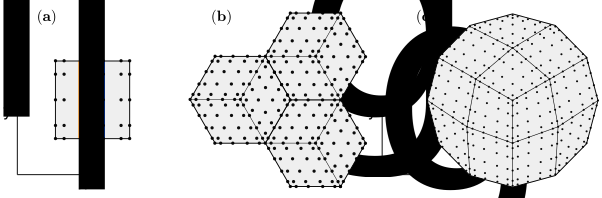
\includegraphics{Chapter_5/skin_mesh}
	\end{center}
	\caption{The mesh with the node distribution, (\textbf{a}) spectral element used for modeling the wall of the core, (\textbf{b}) excerpt of the skin plate and (\textbf{c}) cyanoacrylate glue mesh with the second-order curve at the boundary.}
	\label{fig:skin_mesh}
\end{figure}

The convergence of the solution requires time increment to be less than a critical value, above which the displacements go to infinity.
In the present model, convergence was achieved for \(\Delta t=\)\num{12.2e-3} \(\mu\)s.
The number of nodes for the particular elements are as follows: the core \(6 \times 5\), epoxy adhesive and cyanoacrylate glue \(6 \times 6\), the plate \(6 \times 6 \times 4\) and \acp{pzt} \(6 \times 6 \times 3\).
While the max length of the skin element is six mm, such a \ac{cfrp} model satisfies the condition of at least six nodes per wavelength for the \ac{a0}, as it is the shortest mode propagating in the assumed frequency range.
Table~\ref{tab:wavelength} shows the \ac{a0} wavelengths for various frequency and propagation angles.
\begin{table}[H]
	\small
	\tabcolsep=0.75cm
	%\centering
	\caption{\label{tab:wavelength}The wavelength of the \ac{a0} mode propagated in the presented \ac{cfrp} plate.}
	\begin{tabular}{cccccc}
		\toprule
		\textbf{Frequency} & \multicolumn{5}{c}{\textbf{Propagation angle}}\\
		kHz & \(0^{\circ}\) & \(30^{\circ}\) & \(45^{\circ}\) & \(60^{\circ}\) & \(90^{\circ}\)\\
		\midrule
		50 & 16.5& 15.2&15.0&15.2&16.6\\
		100 & 10.3& 9.6&9.5&9.6&10.3\\
		150 & 7.5& 7.1&7.0&7.1&7.5\\
		\bottomrule
		\multicolumn{6}{r}{{\scriptsize{source: Dispersion Calculator v1.9}}}
	\end{tabular}
\end{table}
%% SECTION HEADER /////////////////////////////////////////////////////////////////////////////////////
\section{\Acf{hcgm}}
\label{sec:homogenised}

%% SECTION CONTENT ////////////////////////////////////////////////////////////////////////////////////
In the section \ref{sec:modelling}, several examples are given of the successful application of the model to numerical analysis of \ac{gw} propagation and damage localisation in \ac{hsc}.
Its unquestionable advantage is the simplified component mesh, reducing operating memory resources.
In dissertation, comparative studies between the \ac{hcgm} and the \ac{fcgm} was conducted to assess the simplified model effectiveness in estimating damage size.

In the \ac{hcgm}, the values of the material constants of the panel core were calculated according to the method presented by Malek and Gibson \cite{malek2015effective}.
This model is an extension of the theoretical analysis of Gibson et al. \cite{gibson1982mechanics}, considering the different geometry of the cell and the nodes at the intersection of the vertical and inclined walls.

The comprehensive formulation of the stiffness matrix components is given in App.~\ref{app:eff_properties} and the effective mechanical properties are gathered in Table \ref{tab:properties_eff}.
The properties for other structures, i.e., the skin, the epoxy adhesive, the cyanoacrylate glue, and the sensors remained unchanged.
The core element has \(6 \times 6 \times 4\) nodes, and the mesh coincides with the skin mesh.
The elements of the other structures are the same as described in the previous section.
%% SECTION HEADER /////////////////////////////////////////////////////////////////////////////////////
\section{Damaged structure implementation}
\label{sec:disbond}
%% SECTION CONTENT ////////////////////////////////////////////////////////////////////////////////////
The skin and the core disbonds were evaluated to analyse the effect of damage on GW propagation.
A rectangular region of disbonds was investigated with the length along the wave propagation varying in width \(\mathrm{w_d} = [0,10,30,50,70,100,120]\) mm, and the damage length in the perpendicular direction was constant \(\mathrm{l_d} = 170\) mm.
The rectangle was centrally located between the transducers, as presented in Figure~\ref{fig:honeycomb}(\textbf{a}).
The selected dimensions of the defects correspond to the dimensions of disbonds made in the specimen to be measured experimentally.
The damage was done with a sharp hooked tool that detached the core from the adhesive layer cell by cell.
The dimensions of the disbond had a coarse tolerance, measuring the width by a calliper.
Due to the small aluminium sheet thickness, the core cells were squashed within the damaged area as it can be seen in Figure~\ref{fig:disbond}\textbf{(a)}.

Two kinds of disbond models were considered in the analysis.
The core cells were removed from the damaged area in the first model as in the mesh pictured in Figure~\ref{fig:disbond}(\textbf{b}).
Whereas in the second model, all components were intact, and only the interface elements between the adhesive layer and the core were decoupled within the yellow area indicated in Figure~\ref{fig:disbond}(\textbf{c}).
\begin{figure}[!bh]
	\begin{center}
		\includegraphics[width=0.9\textwidth]{Chapter_5/disbond}
	\end{center}
	\caption{The damaged area in the: (\textbf{a}) experimental sample,(\textbf{b}) numerical model with removed cells and (\textbf{c}) numerical model with interface decoupling}
	\label{fig:disbond}
\end{figure}
%% SECTION HEADER /////////////////////////////////////////////////////////////////////////////////////
\section{Convergence tests of the solution}
\label{sec:convergence}

%% SECTION CONTENT ////////////////////////////////////////////////////////////////////////////////////

\subsection{Spatial convergence}
Spatial convergence was determined after simulations for samples with elements of different order of the Legendre polynomial (see Eq. \ref{eq:nodes}).
The polynomial order for the \(\xi\times \eta\) plane in the local reference system were changed in the set: \(p=[4,\,5,\,7,\,9,\, 11]\).
The exact order was assumed for each component to minimise the non-zero value of coupling matrix \(\textbf{G}\).
Due to the perpendicularity of the core elements to the skin, the nodes along the core thickness are fixed to 5.
As a criterion for convergence, the percentage error defined as:
\begin{eqnarray}
	\delta^{\mathrm{conv}} = \frac{\sum{\left(e^{\mathrm{max}}-e^{p}\right)^2}}{\sum{\left(e^{max}\right)^2}} \times 100\%,
	\label{eq:perc_err_conv}
\end{eqnarray}
where \(e^{max}\) and \(e^{p}\) are the signal envelopes for the case with the elements of \(11^{\mathrm{th}}\) polynomial order and the observed case, respectively.
A 5\% threshold was assumed for choosing the degree of the polynomial.
The signal envelope is obtained using the Hilbert transform, which is defined as \cite{staszewski2004health}:
\begin{eqnarray}
	\label{eq:hilbert}
	\hat{x}(t) &=& \frac{1}{\pi}\int_{-\infty}^{+\infty}x(\tau)\frac{1}{t-\tau}\diff\tau,\\
	\label{eq:envelope}
	e(t) &=& \sqrt{x^2(t)+\hat{x}^2(t)}.
\end{eqnarray}
\nomtypeD[e]{\(e(t)\)}{Signal envelope}{}%
\nomtypeR[t]{\(t\)}{Time vector}{}{\unit{\second}}%

The example of the simulated signals of 100 \unit{\kHz} are presented in Fig. \ref{fig:dx_conv}\textbf{(a)}.
It can be seen that despite the good agreement of the wave speed for all cases, the amplitudes converge only for a polynomial of order 7.
Based on the graph showing simulation errors (Fig. \ref{fig:dx_conv}(\textbf{b})), the polynomial of order \(p=7\) was selected for 50 and 100 \unit{\kHz} signals, and order \(p=9\) was selected for the 150 \unit{\kHz} signal.
 
Tab \ref{tab:elements_nodes} contains a complete list of elements with the number of nodes on each axis \(\xi\times \eta \times \zeta\) which were assumed in simulations.
\begin{figure}[H]
	\begin{center}
		\includegraphics[width=0.95\textwidth]{Chapter_5/dx_conv}
	\end{center}
	\caption{Spatial convergence for the sample, \textbf{(a)} the sensor signals of 100 \unit{\kHz} for various number of the in-plane nodes (\(n \times m\)) of the element, \textbf{(b)} percent error for the differ polynomial order}
	\label{fig:dx_conv}
\end{figure}
\begin{table}[H]
	\small
	\tabcolsep=0.5cm
	\centering
	\caption{\label{tab:elements_nodes}The node numbers of the sample components.}
	\begin{tabular}{cccc}
		\toprule
		\multirow{3}{*}{\textbf{Component}} & \multicolumn{3}{c}{\textbf{Number of element nodes}}\\
		& \multicolumn{3}{c}{\(n\times m \times l\)}\\
		& 50 \unit{\kHz} & 100 \unit{\kHz} & 150 \unit{\kHz}\\
		\midrule
		Core & \multicolumn{2}{c}{\numproduct{8 x 5 x 1}} & \numproduct{10 x 5 x 1}\\
		Adhesive layer & \multicolumn{2}{c}{\numproduct{8 x 8 x 1}} & \numproduct{10 x 10 x 1}\\
		Skin & \multicolumn{2}{c}{\numproduct{8 x 8 x 4}} & \numproduct{10 x 10 x 1}\\
		Glue & \multicolumn{2}{c}{\numproduct{8 x 8 x 1}} & \numproduct{10 x 10 x 1}\\
		\ac{pzt} & \multicolumn{2}{c}{\numproduct{8 x 8 x 3}} & \numproduct{10 x 10 x 3}\\
		\bottomrule
	\end{tabular}
\end{table}

While the maximum length of the skin element is 6 \unit{\mm}, such a \ac{cfrp} model satisfies the condition of at least six nodes per wavelength for the \ac{a0}, as it is the shortest mode propagating in the assumed frequency range.
Table~\ref{tab:wavelength} shows the \ac{a0} wavelengths for various frequency and propagation angles.
\begin{table}[H]
	\small
	\tabcolsep=0.75cm
	%\centering
	\caption{\label{tab:wavelength}The wavelength of the \ac{a0} mode propagated in the presented \ac{cfrp} plate.}
	\begin{tabular}{cccccc}
		\toprule
		\textbf{Frequency} & \multicolumn{5}{c}{\textbf{Propagation angle}}\\
		\unit{\kHz} & \ang{0} & \ang{30} & \ang{45} & \ang{60} & \ang{90}\\
		\midrule
		50 & 16.5& 15.2&15.0&15.2&16.6\\
		100 & 10.3& 9.6&9.5&9.6&10.3\\
		\bottomrule
		\multicolumn{6}{r}{{\scriptsize{source: Dispersion Calculator v1.9}}}
	\end{tabular}
\end{table}
\subsection{Temporal convergence}
A temporal convergence test is conducted to select the appropriate time step value.
The critical value of time increment (\(\Delta t_{cr}\)) depends on the mesh size and the wave mode velocity.
If this value is set over (\(\Delta t_{cr}\)), the displacement of the structure will increase to infinity in the initial moments of the simulation as it is presented in Fig. \ref{fig:dt_cr}.
This indicates that the time step have to be further decreased which can be easy implemented for testing of the stability of the method.
\begin{figure}[!tbh]
	\begin{center}
		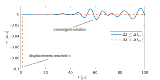
\includegraphics[width=0.95\textwidth]{Chapter_5/dt_cr}
	\end{center}
	\caption{The displacement of the plate at a point of 50 mm away from actuator in the case of correctly and incorrectly selected time increments.}
	\label{fig:dt_cr}
\end{figure}


\section{Conclusions}
\label{sec:conclusionsSimul}

The Chapter describes the whole model configuration for numerical simulations.
The mesh generation for each component, the excitation signals, and the description of damage modelling are included.
A comparison between the \ac{fcgm} and \ac{hcgm} is also provided.

An essential issue in numerical modelling is the convergence of the solution in the spatial and temporal domains.
Incorrectly selected model parameters cause significant errors in the results.
When a time increment is set over the critical value, displacements tend immediately to infinity.
The size and order of the spectral element should be selected depending on the smallest propagating wavelength in the analysed structure.
In turn, the smallest distance between nodes affects the critical value of the time step.
All this has a consequence on the duration of computer simulations.
% Note that the text in the [] brackets is the one that will
% appear in the table of contents, whilst the text in the {}
% brackets will appear in the main thesis.

%% CHAPTER HEADER /////////////////////////////////////////////////////////////////////////////////////
\chapter[Experimental Validation]{Experimental Validation}
\label{ch:validation}

%% CHAPTER INTRODUCTION ///////////////////////////////////////////////////////////////////////////////


%% INCLUDE SECTIONS ///////////////////////////////////////////////////////////////////////////////////

%%% SECTION HEADER /////////////////////////////////////////////////////////////////////////////////////
\section{Experimental Setup Configuration}
\label{sec:setup}

%% SECTION CONTENT ////////////////////////////////////////////////////////////////////////////////////

The presented model was validated with results from two experimental studies.
The first one was performed for determination of the full wavefield of the propagating waves by the \ac{sldv} (Polytec PSV–400).
The second study was performed for wave acquisition by the \ac{pzt} sensor.
The schematic of the experimental setup is shown in Figure~\ref{fig:setup}.
The sample of interest was a not-regular hexagonal aluminium honeycomb bonded to one \ac{cfrp} plate  using the epoxy adhesive (Loctite EA3479B) as shown in Figure~\ref{fig:honeycomb}(\textbf{a}).%PF: label acc. to figure caption.
The subject of the parametric study was the effect of the disbond size on the propagating GW.

\begin{figure}[H]
	%	\begin{center}
	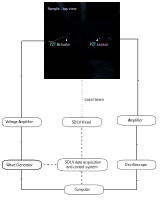
\includegraphics[width=1\linewidth]{Chapter_6/setup}
	%	\end{center}
	\caption{Experimental setup for the (1) \ac{sldv} measurement---dashed line and (2) PZT wave acquisition---solid line.}
	\label{fig:setup}
\end{figure}
\vspace{-12pt}
\begin{figure}[H]
	%	\begin{center}
	\includegraphics[width=1\linewidth]{Chapter_6/honeycomb}
	%	\end{center}
	\caption{Sample configuration: (\textbf{a}) top view of the sample, (\textbf{b}) honeycomb sandwich substructures and (\textbf{c}) details of the honeycomb cell.}
	\label{fig:honeycomb}
\end{figure}


After a reference measurement was made on an intact sample, several measurements were taken for the subsequent damage introduced on the same specimen.
The circular area of the core was detached from the adhesive at the center of the plate using a sharp hooked tool.
For this purpose, the bottom skin was omitted so that damage could be introduced.
The damage size was controlled by its diameter \(\Phi_D=\left [10, 30, 50, 70, 90, 110, 130 \right ]\) mm.

The generation and reception of elastic waves were achieved with a pair of \ac{pzt} transducers mounted on the skin top surface with the cyanoacrylate glue.
The coordinates of the actuator were \((x_1,y_1)=(-100,0)\) mm,	and for the sensor, \((x_2,y_2)=(100,0)\) mm.
The dimensions of the sample components were as follows:
\begin{itemize}
	\item \ac{cfrp} skin: \(L \times W \times H = 500 \times 500\ \times 1.5\) mm,
	\item Aluminium core: \(g=14.5\) mm, \(w=0.1\) mm, \(h_1=11\) mm, \(h_2=5\) mm, \(l_1=10.4\) mm, \(l_2=6\) mm,
	\item Epoxy adhesive: \(L\times W \times H = 500 \times 500 \times 0.3\) mm,
	\item NCE51 \ac{pzt}: \(\Phi_{PZT}=10\) mm, \(h=0.5\) mm,
	\item Cyanoacrylate glue: \(\Phi_{CG}=10\) mm, \(h=0.05\) mm.
\end{itemize}

The \(N_c=5\) cycle Hann windowed signal at carrier frequencies \mbox{\(f_c=[75,100,125,150]\) kHz} was generated using an arbitrary waveform generator (National Instruments, PXI 5413).
The signal was amplified 40 times and supplied to the \ac{pzt} actuator (Noliac, NCE51).
Each measurement was conducted in the room temperature and averaged 20~times in order to improve the signal to noise ratio.
%%% SECTION HEADER /////////////////////////////////////////////////////////////////////////////////////
\section{Results}
\label{sec:resuls}
%% SECTION CONTENT ////////////////////////////////////////////////////////////////////////////////////
\subsection{\acs{hsc} validation with \acs{sldv} setup}
The full wavefield in the reference sample is presented in Fig.~\ref{fig:wavefield}.
The experimental measurements and the \ac{fcgm} snapshots show that the wavefront distortion is rising with the frequency.
Because the wavelength decreases as the frequency increases, a higher frequency signal is more likely to reflect off the core walls.
This effect is not observed in the case of the \ac{hcgm}.
\vspace{-6pt}
\begin{figure}[H]
	\begin{center}
		\includegraphics[width=0.95\textwidth]{Chapter_6/fullfield}
	\end{center}
	\caption{The top surface out of plane particle velocity snapshots in the time 100 \unit{\micro\second} for (\textbf{a}) the experimental results obtained by using the \acf{sldv}, (\textbf{b}) the \acf{fcgm} and (\textbf{c}) the \acf{hcgm} in the healthy~sample.}
	\label{fig:wavefield}
\end{figure}

\begin{figure}[H]
	\begin{center}
		\includegraphics[width=0.95\textwidth]{Chapter_6/fullfield_dam}
	\end{center}
	\caption{The top surface out of plane particle velocity snapshots in the time 100~\unit{\micro\second} for (\textbf{a}) the experimental results obtained by using \ac{sldv} in the sample with 90 \unit{\mm} width damage, (\textbf{b}) the \acf{fcgm} and (\textbf{c}) the \acf{hcgm} with removed core elements in damaged area for both numerical models.}
	\label{fig:wavefield_dam5}
\end{figure}

In case of the damaged sample, the wavefront is not distorted in the damage area bounded by two dotted lines in Fig.~\ref{fig:wavefield_dam5} for all three cases.
Due to the lack of wave leakage into the core, the wave propagates smoothly through the skin.
For the experimental sample and the \ac{fcgm}, interference of waves reflected from the cells and the damage boundary is observed.
The wave interference observed in the \ac{hcgm} refers to waves reflected only from the defect.

\subsection{\acs{hsc} validation with \acsp{pzt} wave acquisition setup}
Validation of the honeycomb structure models and a separate \ac{cfrp} plate intended for the \ac{hsc} sample were done by comparing the group velocity and amplitude of the first packet of \ac{s0} and \ac{a0} arriving at the sensor.
In the Fig.~\ref{fig:signal_exp_raw} are presented examples of the experimentally obtained raw signals for the healthy and damaged samples.
The raw signals are processed for noise reduction and determine an envelope of the signals.
The envelope is used to obtain the amplitude and group velocity of the mods for the model validation and will be used in the analytical assessment of damage magnitude.
\begin{figure}[H]
	\begin{center}
		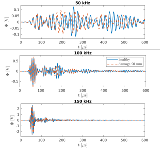
\includegraphics[width=0.95\textwidth]{Chapter_6/signal_exp_raw}
	\end{center}
	\caption{Raw signals registered by the sensor in \acf{hsc} for healthy and damage of 90 \unit{\mm} width.}
	\label{fig:signal_exp_raw}
\end{figure}

Signal processing follows the diagram shown in Fig.~\ref{fig:signal_processing}.
A preliminary step is a conversion of the signals from the time domain to the frequency domain by the \ac{fft}.
Then, the pass-band filter attenuates the frequencies outside of the range \(0.5f_c-1.5f_c\).
A Butterworth filter of 20th order was used.
After filtering the signal is again converted to the time domain by the \ac{ifft}.
Lastly, the envelope of the signal \(e(t)\) is obtained using the Hilbert transform \(\hat{x}(t)\). The definition of both operators given in the book \cite{staszewski2004health} is defined as follows:
\begin{eqnarray}
	\hat{x}(t) &=& \frac{1}{\pi}\int_{-\infty}^{+\infty}x(\tau)\frac{1}{t-\tau}\diff\tau,\\
	e(t) &=& \sqrt{x^2(t)+\hat{x}^2(t)}.
\end{eqnarray}

\begin{figure}[H]
	\begin{center}
		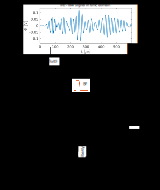
\includegraphics[width=0.95\textwidth]{Chapter_6/signal_processing}
	\end{center}
	\caption{Raw signals registered by the sensor in \acf{hsc} for healthy and damage of 90 \unit{\mm} width.}
	\label{fig:signal_processing}
\end{figure}

The group velocity is derived from the signal envelope determining of the mode \ac{tof}.
The \ac{tof} is a difference between the arrival of the maximum amplitude of the envelope of considered mode at the sensor \((\mathrm{T}_1)\) and the half time of the excitation pulse \(\left(\mathrm{T}_0=\frac{1}{2f_m}\right)\).
Since the distance between the transducers is constant \(l=200\) \unit{\mm}, the group velocity equals:
\begin{eqnarray}
	C_g = \frac{\mathrm{ToF}}{l}=\frac{T_1-T_0}{l}.
\end{eqnarray}
All the experimental signals were processed with the band-pass filter in the frequency range from \(0.5f_c\) to \(1.5f_c\).

The signal envelopes are shown in Fig.~\ref{fig:single_skin} for single \ac{cfrp} plate, Fig.~\ref{fig:hsc_full} for \ac{fcgm}, and Fig.~\ref{fig:hsc_homo}, from which the velocities and amplitudes of the wave mods were determined.
\begin{figure}[H]
	\begin{center}
		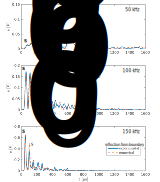
\includegraphics[width=0.95\textwidth]{Chapter_6/single_skin}
	\end{center}
	\caption{The signal envelope for single \acf{cfrp} skin; experimental vs. numerical simulation.}
	\label{fig:single_skin}
\end{figure}
\begin{figure}[H]
	\begin{center}
		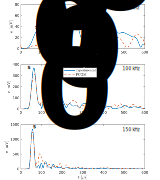
\includegraphics[width=0.95\textwidth]{Chapter_6/HSC_full}
	\end{center}
	\caption{The signal envelope for the \acf{hsc} structure; experimental vs. \acf{fcgm}.}
	\label{fig:hsc_full}
\end{figure}
\begin{figure}[H]
	\begin{center}
		\includegraphics[width=0.95\textwidth]{Chapter_6/HSC_homo}
	\end{center}
	\caption{The signal envelope for the \acf{hsc} structure; experimental vs. the \acf{hcgm}.}
	\label{fig:hsc_homo}
\end{figure}

For the single \ac{cfrp} plate, Tab. \ref{tab:group_velocity_cfrp} gives the determined velocities and amplitudes of the modes together with the percentage errors defined as:
\begin{eqnarray}
	\delta = \left|\frac{x^{num}-x^{exp}}{x^{exp}}\right|\times100\%,
\end{eqnarray}
where \(x^{num}\) and \(x^{exp}\) are the numerical and experimental values, respectively.
It can be noticed that the model are in good agreement with experimental results.
All values are within an error of up to 10\%, except for the \ac{s0} and \ac{a0} amplitudes for 50 and 100 \unit{\kHz}, respectively.
For these cases, the error is about 25\%.
There is no data for the \ac{a0} of 150 \unit{\kHz}, as the high amplitude \ac{s0} reflections mask it.

Regarding the \ac{hsc} panel, best results are achieved for the \ac{fcgm} as it is shown in Tab.~\ref{tab:group_velocity_hsc}.
The velocity error is less then 16.4\% for both modes. 
In the case of amplitude values, only the \ac{s0} of 50 \unit{\kHz} and the \ac{a0} of 100 \unit{\kHz} are overestimated by the model with the error around 25 \%.
For the \ac{hcgm}, best result are obtained for the 100 \unit{\kHz}. 
The velocity error is about 5\% for both modes. 

\begin{table}[H]
	\small
	\tabcolsep=0.2cm
	\centering
	\caption{\label{tab:group_velocity_cfrp} Comparison between of the modes amplitudes and group velocities obtained from the simulations and experiments for the single \acf{cfrp} plate.}
	\begin{tabular}{cccccccc}
		\toprule
		& & \multicolumn{3}{c}{\(C_g\)} & \multicolumn{3}{c}{Amp.}\\
		\multirow{2}{*}{Mode} & Frequency & Exp. & Num. & \(\delta\)& Exp. & Num. & \(\delta\)\\
		& \unit{\kHz} & \unit[per-mode = symbol]{\m\per\s} & \unit[per-mode = symbol]{\m\per\s} & \% & \unit{\mV} & \unit{\mV} & \% \\
		\midrule
		\multirow{3}{*}{\ac{s0}} & 50 & 6079 & 5865 & \textcolor{green}{3.52}& 12 & 171 & \textcolor{red}{25.0} \\
		&100& 5571 & 5747 & \textcolor{green}{3.16} & 171 & 162 & \textcolor{green}{5.26}\\
		&150& 5764 & 5698 & \textcolor{green}{1.15} & 648 & 664 & \textcolor{green}{2.47}\\
		\midrule
		\multirow{3}{*}{\ac{a0}} &50& 1341 & 1325 & \textcolor{green}{0.74} & 134 & 125 & \textcolor{green}{6.72}\\
		&100& 1550 & 1396 & \textcolor{green}{9.74} & 84 & 104 & \textcolor{red}{23.8}\\
		&150& \multicolumn{6}{c}{-} \\
		\bottomrule
	\end{tabular}
\end{table}
\begin{table}[H]
	\small
	\tabcolsep=0.15cm
	\centering
	\caption{\label{tab:group_velocity_hsc} Comparison between of the modes amplitudes and group velocities obtained from the simulations based on \acf{fcgm} and \acf{hcgm} and experiments for \acf{hsc}.}
	\begin{tabular}{cccccccccccc}
		\toprule
		& & \multicolumn{5}{c}{\(C_g\)} & \multicolumn{5}{c}{Amp.}\\
		\multirow{2}{*}{Mode} & Freq.& Exp. & \ac{fcgm} & \(\delta\) & \ac{hcgm} & \(\delta\) &  Exp. & \ac{fcgm} & \(\delta\) & \ac{hcgm} & \(\delta\)\\
		& \unit{\kHz} & \unit[per-mode = symbol]{\m\per\s} & \unit[per-mode = symbol]{\m\per\s} & \% & \unit{\mV} & \unit{\mV} & \% & \unit[per-mode = symbol]{\m\per\s} & \%& \unit[per-mode = symbol]{\m\per\s} & \% \\
		\midrule
		\multirow{3}{*}{\ac{s0}} & 50 & 6329 & 5291 & {16.4} & 8230 & 30 & 33 & 12 & \textcolor{red}{63.6} & 3 & \textcolor{red}{90.9} \\
		&100& 5291 & 5249 & \textcolor{green}{0.79} & 5540 & \textcolor{green}{4.71} & 369 & 341 & \textcolor{green}{7.59} & 152 & \textcolor{red}{58.8}\\
		&150& 5031 & 4866 & \textcolor{green}{2.93} & 4301 & 14.4 & 1340 & 1056 & {21.2} & 359 & \textcolor{red}{73.8} \\
		\midrule
		\multirow{3}{*}{\ac{a0}} & 50 & 964 & 945 & \textcolor{green}{1.97} & 1318 & 36.7 & 62 & 57 & \textcolor{green}{8.06} & 70 & 12.9\\
		& 100 & 2160 & 2075 & \textcolor{green}{3.94} & 2273 & \textcolor{green}{5.23} & 137 & 249 & \textcolor{red}{81.8} & 128 & \textcolor{green}{6.57}\\
		& 150 & \multicolumn{10}{c}{-}\\
		\bottomrule
	\end{tabular}
\end{table}
Errors in the models may be due to several factors.
The most important ones include differences in material properties of used components.
In the models, an average thickness of the adhesive layer was assumed; obtaining precise thickness of the adhesive layer in the specimen preparation is difficult under workshop conditions.
The models also assume a uniform cell geometry for the core area, but in reality, the core is easily deformed in the plane, so the cell geometry varies.
The velocity in the \ac{cfrp} plate varies with the angle of propagation; in the models, the direction of wave propagation between the sensors was assumed to coincide with the plate orientation.
The speed is also affected by the accuracy of the \acp{pzt} placement.
\subsection{Efficiency of the time integration algorithm}
Two types of simulations were conducted to determine the efficiency of the \ac{pa} to solve the equation of motion shown in Section \ref{sec:gpu}.
The first type compares the \ac{pa} computations performed on the \ac{gpu} and \ac{cpu}.
The second type compares \ac{pa} with the benchmark proposed by Kudela et al.~\cite{kudela2020parallel} named \ac{ba}.
Both analyses were performed on the same workstation as the \ac{ba} equipped with the following components:
\begin{itemize}
	\item \ac{cpu} - Intel Xeon Silver, 2.1 \unit{\giga\Hz}, 8 cores
	\item \ac{gpu} - NVIDIA Tesla V100 32 \unit{\giga\byte} 5120 CUDA cores
	\item RAM - 128 \unit{\giga\byte} DDR4 2933 \unit{\mega\Hz}
\end{itemize}

The comparison \ac{gpu} vs. \ac{cpu} was conducted on a \ac{3d} model of an  aluminium plate (\numproduct{250 x250 x 5} \unit{\cubic\mm}).
The structure was discretised with rectangular mesh of the various number of the in-plane elements.
In each case, a spectral element of \numproduct{6 x 6 x 3} nodes with three \acp{dof} per node was used, with one element through the plate thickness.
The global \ac{dof} and the memory usage are presented in Table~\ref{tab:gpuvscpu}.
A concentrated force was applied to the centre of the plate as a 3-cycle Hann windowed sine at 50 \unit{\kHz} frequency.
\begin{table}[!b]
	\tabcolsep=0.2cm
	\centering
	\caption{\label{tab:gpuvscpu} Model parameters used in simulations to compare the algorithm performed on \ac{gpu} and \ac{cpu}.}
	\begin{tabular}{lccccc}
		\toprule
		Number of elements & \numproduct{25 x 25} & \numproduct{50 x 50} & \numproduct{100 x 100} & \numproduct{125 x 125} & \numproduct{250 x 250} \\
		Global \ac{dof}\(\times10^6\) &0.14&0.57&2.26&3.53&14.08\\
		Memory usage \unit{\mega\byte} & 75 & 367 & 1437 & 2252 & 8999\\ \bottomrule
	\end{tabular}
\end{table}
The computational speed up as a function of global \ac{dof} was determined as follows:
\begin{eqnarray}
\mathrm{Speedup} = \frac{\mathrm{CPU_{avg}}}{\mathrm{GPU_{avg}}},
\end{eqnarray}
where \(\mathrm{CPU_{avg}}\) and \(\mathrm{GPU_{avg}}\) is average one time step calculation performed on \ac{cpu} and \ac{gpu}, respectively.
The time of the pre-/post-processing is not included into the speedup calculation, because the data from \ac{cpu} to \ac{gpu} and vice versa is done only once, while the time integration steps are a large number. 

For the second test computations run times of the simulations conducted on \ac{gpu} were computed for various sizes of the composite plate.
The benchmark parameters proposed in the paper mentioned above are gathered in Table~\ref{tab:benchmark}.
The efficiency of the \ac{pa} regarding \ac{ba} is measured by speedup, defined as the ratio of \ac{ba} run time to \ac{pa}.
\begin{table}[!t]
\tabcolsep=0.2cm
\centering
\caption{\label{tab:benchmark}Sample parameters used in the benchmark of the \ac{pa} and the \ac{ba}.}
	\begin{tabular}{lcccccc}
		\toprule
		Plate size \unit{\cm} & \numproduct{30 x 30} & \numproduct{40 x 40} & \numproduct{50 x 50} & \numproduct{70 x 70} & \numproduct{90 x 90} & \numproduct{100 x 100}\\
		Global \ac{dof}\(\times10^6\)&1.02&1.46&1.98&3.09&5.23&6.36\\ \bottomrule
	\end{tabular}
\end{table}

The results of both analysis are pictured in Fig.~\ref{fig:speedup}.
At maximum \ac{dof}, the speedup in \ac{gpu} computation relative to \ac{cpu} computation increases near to 90 and the \ac{pa} is up to ten times more efficient than the \ac{ba}.
Improvement of the algorithm comes from: more operations performed in the preprocessing, transfer of internal forces from the local to the global system by summing columns instead of \verb+for-loop+, and minimized number of columns in the map of local nodes $\textbf{I}_L$ (see section~\ref{sec:gpu}).
\begin{figure}[!tbh]
	\begin{center}
		\includegraphics[width=0.95\textwidth]{Chapter_6/benchmark}
	\end{center}
	\caption{Speedup in function of global \acfp{dof} of the \acf{pa} computation run on \acf{cpu}~vs.~\acf{gpu} dashed line, and compared to \acf{ba} solid line}
	\label{fig:speedup}
\end{figure}
%%% SECTION HEADER /////////////////////////////////////////////////////////////////////////////////////
\section{Conclusions}
\label{sec:conclusionsValid}

%% SECTION CONTENT ////////////////////////////////////////////////////////////////////////////////////
This chapter presents the experimental validation of the \ac{fcgm} and \ac{hcgm}.
It is shown that the \ac{fcgm} better expresses the wave propagation in \ac{hsc} than the simplified model.
The snapshots of the full wavefield show wave interference in the core cells, which is impossible in the \ac{hcgm}.
The full-field analysis also showed a lack of wave leakage into the core at the damaged area.
This phenomenon will be the basis for determining the effect of the damage on wave propagation.
The velocity of the wave propagation for both models is in good agreement with the \ac{pzt} measurements.
Additionally, it was shown that by optimising the algorithm for solving the equation of motion, a calculation time was achieved ten times faster than the algorithm presented in the paper \cite{kudela2020parallel}.
% Note that the text in the [] brackets is the one that will
% appear in the table of contents, whilst the text in the {}
% brackets will appear in the main thesis.

%% CHAPTER HEADER /////////////////////////////////////////////////////////////////////////////////////
\chapter[Parameter study of \ac{gw} propagation in \ac{hsc}]{Parameter study of \ac{gw} propagation in \ac{hsc}}
\label{ch:tempEffects}

%% CHAPTER INTRODUCTION ///////////////////////////////////////////////////////////////////////////////
In the chapter~\ref{ch:severity}, the \ac{madif} was determined for the sample at ambient temperature of \(+20^{\circ}\)C.
However, quasi-stable conditions can only be guaranteed in a laboratory.
Therefore, from a practical point of view, it is necessary to consider changes due to different working conditions.
In this chapter, a study will be carried out to determine the effect of various ambient temperatures on the \ac{madif}.
In addition, a series of computer simulations will be performed to determine how the different parameters of the \ac{hsc} components affect the wave propagation in this structure.
The analysis will include factors such as the adhesive thickness, the \ac{pzt} placement regarding the core cell, the core orientation regarding the wave propagation and volume fraction of reinforcing fibres.
Finally, the \ac{madif} will be developed for \ac{hsc} with the skins on the top and bottom sides of the core.
%% INCLUDE SECTIONS ///////////////////////////////////////////////////////////////////////////////////
%% SECTION HEADER /////////////////////////////////////////////////////////////////////////////////////
\section{The \acs{madif} under variable temperature conditions}
\label{sec:madifTemp}

%% SECTION CONTENT ////////////////////////////////////////////////////////////////////////////////////
In addition to the referenced \ac{madif} obtained for +20\unit{\degreeCelsius}, a study of wave propagation at temperatures T=\(\left[-10,\,0,\,+10,\,+30,\,+40,\,+50\right]\)\unit{\degreeCelsius} was carried out.
To determined temperature-dependent simulations of \ac{gw} propagation in \ac{hsc}, the material properties of the components were determined according to the methodology described in section~\ref{sec:temp}.

The temperature effect on the \acp{madif} is developed based on the \ac{fcgm} and removed core cells as a damage model.
The analysis used both \acp{di}, i.e. the \ac{rmsd} and the \ac{cc}, for the 100 \unit{\kHz} full-length signal.
The signal obtained for a healthy sample at each temperature was taken as the reference signal for each case.
\begin{table}[!tbh]
	\small
	\tabcolsep=0.25cm
	\centering
	\caption{\label{tab:fit_F_err_temp} The time-dependent coefficients and errors of the function from Eq.~(\ref{eq:function_1}) fitted to \acp{di} based on the \acf{fcgm} - core.}
\begin{tabular}{c|cc|cc}
	\toprule \multirow{3}{*}{T \unit{\degreeCelsius}} & \multicolumn{2}{c|}{\ac{rmsd}} & \multicolumn{2}{c}{\ac{cc}}\\
	&\multicolumn{2}{c|}{100 \unit{\kHz}}&\multicolumn{2}{c}{100 \unit{\kHz}}\\
	& \(a_i\) &  \(\delta^{\mathrm{fit}}\) \% & \(a_i\) & \(\delta^{\mathrm{fit}}\) \%\\
	\midrule
	 \multirow{3}{*}{0} & 24.72 & \multirow{3}{*}{\textcolor{green}{1.43}}& 123.8 & \multirow{3}{*}{\textcolor{green}{0.48}}\\
	 & 90.62 & & 404.2 &\\
	 & 0.57 & & 0.67 &\\
	\midrule
	\multirow{3}{*}{+10} & 6.37 & \multirow{3}{*}{\textcolor{green}{1.31}}& 42.81 & \multirow{3}{*}{\textcolor{green}{0.43}}\\
	& 24.91 & & 208.3 &\\
	& 0.67 & & 0.78 &\\
	\midrule
	\multirow{3}{*}{+30} & 3.62 & \multirow{3}{*}{\textcolor{green}{1.32}}& 3.10 & \multirow{3}{*}{\textcolor{green}{0.42}}\\
	& 17.38 & & 41.95 &\\
	& 0.71 & & 0.92 &\\
	\midrule
	\multirow{3}{*}{+40} & 2.43 & \multirow{3}{*}{\textcolor{green}{1.38}}& 0.95 & \multirow{3}{*}{\textcolor{green}{0.44}}\\
	& 19.76 & & 22.09 &\\
	& 0.72 & & 0.94 &\\
	\bottomrule
\end{tabular}
\end{table}

The temperature-dependent \acp{madif} based on \ac{rmsd} and \ac{cc} are presented in Fig.\ref{fig:madif_temp_rmsd} and Fig.~\ref{fig:madif_temp_cc}, respectively.
It is observed that the variation in ambient temperature condition can substantially influence the \ac{madif} values.
From Fig.~\ref{fig:madif_temp_rmsd}, it can be seen that the errors increase the higher the absolute difference between ambient and reference temperature.
Therefore, the assumed linear model of the temperature-dependent material properties of the components used in the simulation is not sufficiently accurate with the real object.
It is particularly evident for temperatures of 0\unit{\degreeCelsius} and -10\unit{\degreeCelsius}, where the \ac{madif} for damage size more than 25 \unit{\mm} does not reach the values obtained experimentally.
The best results were achieved for a temperature of +10\unit{\degreeCelsius}, for which the absolute error does not exceed 2 mm over the full range of damage sizes. 
\begin{figure}[!tbh]
	\begin{center}
		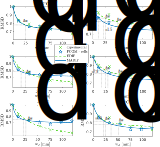
\includegraphics[width=0.95\textwidth]{Chapter_8/MADIF_temp_RMSD}
	\end{center}
	\caption{The \acf{madif} and the \acf{edif} based on the \acf{rmsd} 100 \unit{\kHz}.}
	\label{fig:madif_temp_rmsd}
\end{figure}
\begin{figure}
	\begin{center}
		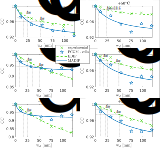
\includegraphics[width=0.95\textwidth]{Chapter_8/MADIF_temp_CC}
	\end{center}
	\caption{The \acf{madif} and the \acf{edif} based on the \acf{cc} 100 \unit{\kHz}.}
	\label{fig:madif_temp_cc}
\end{figure}
%% SECTION HEADER ///////////////////////////////////////////////////////////////////////////////////
\section{The numerical simulation of the \ac{gw} in the \ac{hsc} under various parameters}
\label{sec:parameters}

%% SECTION CONTENT ////////////////////////////////////////////////////////////////////////////////////
In addition to the previous analyses, a parametric study was conducted to determine the effects of various component parameters on \ac{gw} propagation in the \ac{hsc}. The following parameters were taken into account:
\begin{enumerate}
	\item The \ac{pzt} parameters:
	\begin{itemize}
		\item placement in relation to the core cell,
		\item charge constant,
		\item dielectric permittivity,
	\end{itemize}
	\item The \ac{cfrp} and the adhesive layer parameters:
		\begin{itemize}
		\item \ac{cfrp} fibre volume fraction,
		\item adhesive layer thickness,
		\end{itemize}
	\item The core parameters:
	\begin{itemize}
		\item core height and width,
		\item wall thickness,
		\item core rotation angle regarding to wave propagation.
	\end{itemize}
\end{enumerate}

\subsection{The \ac{pzt} parameters}
Computer simulations were conducted to determine the impact of \acp{pzt} placement relative to the core cell.
Seven transducer positions were considered, according to the schematic in Fig.~\ref{fig:pzt_place}(\textbf{b}).
The actuator and sensor position relative to the cell is identical to maintain the same wave propagation distance for each case.

From Fig.~\ref{fig:pzt_place}(\textbf{a}), it can be noticed that the highest amplitude of the \ac{s0} is obtained for the case with the \acp{pzt} placed in the middle of the cell.
The lowest amplitudes were obtained for the cases where the transducer midpoint lay on the core wall.
It is due to the higher stiffness underneath the \ac{pzt}, leading to less displacements.
In the case of the \ac{a0}, the amplitude of the signals for position \#2 and \#5 are much lower than the rest cases.
Since the transducers are permanently fixed to the structure and do not change their position during the monitoring period.
Nonetheless, the \acp{pzt} placement is worth considering to optimise the signals obtained.
\begin{figure}
	\begin{center}
		\includegraphics[width=0.95\textwidth]{Chapter_8/pzt_place}
	\end{center}
	\caption{The \acf{gw} propagation in the \acf{hsc} \textbf{(a)}, sensor responses for \textbf{(b)} different \acf{pzt} placement in relation to the core cell.}
	\label{fig:pzt_place}
\end{figure}

Changes in amplitude under the influence of different values of the piezoelectric charge constant and dielectric permittivity are presented in Fig.~\ref{fig:pzt_d} and ~\ref{fig:pzt_eps}, respectively.
Both parameters have a significant effect on the signal amplitude both the \ac{s0} and \ac{a0}.
The values do not just change with ambient temperature but also degrade over service time \cite{barzegar2001aging, deangelis2006p2o}.
Therefore, I suggest that a sensor self-diagnostic tool should be included in the \ac{shm} system. 
An \ac{emi}-based method could be a good solution as it was suggested for self-diagnostic of damaged transducers by Jiang et al. \cite{jiang2021electromechanical}.

\begin{figure}
	\begin{center}
		\includegraphics[width=0.95\textwidth]{Chapter_8/pzt_d}
	\end{center}
	\caption{The signal envelopes for different piezoelectric charge constants.}
	\label{fig:pzt_d}
\end{figure}

\begin{figure}
	\begin{center}
		\includegraphics[width=0.95\textwidth]{Chapter_8/pzt_eps}
	\end{center}
	\caption{The signal envelopes for different dielectric permittivities.}
	\label{fig:pzt_eps}
\end{figure}

\subsection{The \ac{cfrp} skin and the adhesive layer parameters}

The effect of the skin properties on wave propagation in the \ac{hsc} was analysed for different carbon fibre volume fractions in the composite.
This parameter affects the mode velocity due to the change in effective modulus of elasticity and density of the plate.
A small change in modulus of elasticity leads to significant signal differences within the interference of wave reflections as it can be observe in Fig.~\ref{fig:skin_volume}.
It affects the \ac{madif} determination since the full-length signal is taken into account.

\begin{figure}
	\begin{center}
		\includegraphics[width=0.95\textwidth]{Chapter_8/skin_volume}
	\end{center}
		\caption{Sensor responses in the \acf{hsc} for various fibre volume fractions in the range 45-50\%.}
	\label{fig:skin_volume}
\end{figure}

The effect of the adhesive layer thickness is presented in Fig.~\ref{fig:adhesive_thickness}.
The greater the adhesive thickness, the slower both modes propagate.
There is also a noticeable decrease in the \ac{a0} amplitude, while the \ac{s0} amplitude barely changes.
It is because the \ac{a0} displacements are mainly out-of-plane, so more energy of the wave leaks into the adhesive, and it is attenuated in low-stiffness material.

\begin{figure}
	\begin{center}
		\includegraphics[width=0.95\textwidth]{Chapter_8/adhesive_thickness}
	\end{center}
	\caption{Sensor responses in the \acf{hsc} for various adhesive thicknesses in the range 200-500 \(\mu\)m.}
	\label{fig:adhesive_thickness}
\end{figure}

\subsection{The core parameters}
In the study of the core geometry influence on wave propagation in \ac{hsc}, four parameters were considered:
\begin{itemize}
	\item core height \(g=[10.5,\,12.5,\,14.5,\,16.5,\,18.5]\) \unit{\mm};
	\item core width \(l_1=[5.0,\,6.0,\,7.0,\,8.0,\,9.0]\) \unit{\mm};
	\item wall thickness \(w_c=[100,\,150,\,200,\,250,\,300]\) \unit{\micro\m};
	\item core rotation angle regarding to wave propagation [\ang{0}, \ang{15}, \ang{30}, \ang{45}, \ang{60}, \ang{75}, \ang{90}].
\end{itemize}

From the signal envelopes shown in Fig.~\ref{fig:core_height}, \ref{fig:core_size}, \ref{fig:core_thickness} and \ref{fig:core_rotation} it can be seen that the analysed parameters mainly affect the \ac{a0}. 
In contrast, for the \ac{s0}, only the amplitude changes, except for the reduction in velocity by the increase in wall thickness.

It should be mentioned that all parameters are invariable during the use of the structure and are independent of changing environmental conditions.
Therefore, the core heights and wall thicknesses are set with the dimensions tolerance received from the supplier.
The cell can easily be deformed before bonding to the skin due to the low in-plane stiffness of the core.
Thus for better accuracy, the cell width can be assumed as an average measurement value taken after joining the core with the skin.
The angle of rotation can also be corrected after the components bonding.
\begin{figure}
	\begin{center}
		\includegraphics[width=0.95\textwidth]{Chapter_8/core_height}
	\end{center}
	\caption{Sensor responses in the \acf{hsc} for the various core heights in the range 10.5-18.5 \unit{\mm}.}
	\label{fig:core_height}
\end{figure}

\begin{figure}
	\begin{center}
		\includegraphics[width=0.95\textwidth]{Chapter_8/core_size}
	\end{center}
	\caption{Sensor responses in the \acf{hsc} for the various cell widths in the range 5.0-9.0 \unit{\mm}.}
	\label{fig:core_size}
\end{figure}

\begin{figure}
	\begin{center}
		\includegraphics[width=0.95\textwidth]{Chapter_8/core_thickness}
	\end{center}
	\caption{Sensor responses in the \acf{hsc} for the various wall thicknesses in the range 100-300 \unit{\micro\m}.}
	\label{fig:core_thickness}
\end{figure}

\begin{figure}
	\begin{center}
		\includegraphics[width=0.95\textwidth]{Chapter_8/core_rotation}
	\end{center}
	\caption{Sensor responses in the \acf{hsc} for the various core orientations.}
	\label{fig:core_rotation}
\end{figure}

\subsection{The \ac{madif} for the double-skin \ac{hsc}}

Finally, computer simulations were conducted to determine the \ac{madif} for a structure with a core between two skins.
The single-skin \ac{fcgm} from the previous analyses was supplemented with a \ac{cfrp} plate and also bonded to the core by the adhesive layer.
Two transducers were attached to the top skin as before.
Due to the impossibility of enlarging the damage in a closed-form structure, no experimental measurements were carried out.
Two damage cases were considered in the simulations: (i) interface elements removed from the upper side (the skin with the sensor attached), and (ii) interface elements removed from the bottom side.

Fig.~\ref{fig:madif_2skins}\textbf{(a)} presents the \ac{rmsd}-based \ac{madif} for a double-skin panel with the functions obtained for a single-skin for comparison.
Substantial differences between the double- and single-skin panels can be observed.
In addition, the placement of the damage has also influence on the index slope.
Similar changes in the \ac{madif} can be observed for \ac{cc}, as shown in Fig. ~\ref{fig:MADIF_2skins}\textbf{(b)}.
Although to a lesser extent than the previous index. 
The \ac{rmsd} values ratio single- to double-skin panel for the most significant damage is about 1.5, while the relevant ratio based on \ac{cc} is about 1.08.
\begin{figure}
	\begin{center}
		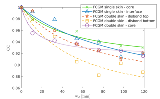
\includegraphics[width=0.95\textwidth]{Chapter_8/MADIF_2skins}
	\end{center}
	\caption{Comparison of the \acf{madif} for single-skin and double-skin panels based on \textbf{(a)}the \acf{rmsd} and \textbf{(b)} the \acf{cc}.}
	\label{fig:madif_2skins}
\end{figure}
\section{Conclusions}
\label{sec:conclusionsTemp}
This chapter presented a parametric study to obtain temperature-dependent \ac{madif} and determine the influence of various parameters of structural components on \ac{gw} propagation in \ac{hsc}.

The \ac{madif} obtained numerically for different ambient temperatures agree very well with the experimental results, especially for temperatures around the reference one.
The absolute error increases with the higher difference in temperature.
It is probably because the assumed linear model is not sufficient enough.

During the analysis, it was shown that the phenomenon of elastic wave propagation in the \ac{hsc} is very complex, and the amplitude value and velocity of the wave strongly depends on many parameters of individual components, signal excitation and environmental conditions.
In the future, it would be essential to develop an optimisation method to determine the material properties and geometry of the structure in order to fit the model to the monitored sample more accurately.
Such a tool based on a genetic algorithm has been developed for a woven fabric reinforced composites by Kudela et al. \cite{kudela2020elastic}.

Computer simulations were also conducted to determine the \ac{madif} for a double-skin structure.
The function, similar to that of a single-skin panel, satisfies the conditions for damage estimation.
% Note that the text in the [] brackets is the one that will
% appear in the table of contents, whilst the text in the {}
% brackets will appear in the main thesis.

%% CHAPTER HEADER /////////////////////////////////////////////////////////////////////////////////////
\chapter[The Severity of Damage Estimation]{The Severity of Damage Estimation}
\label{ch:severity}

%% CHAPTER INTRODUCTION ///////////////////////////////////////////////////////////////////////////////

%% INCLUDE SECTIONS ///////////////////////////////////////////////////////////////////////////////////

%%% SECTION HEADER /////////////////////////////////////////////////////////////////////////////////////
\section{Model-Assisted Damage Identification Function}
\label{sec:madif}

%% SECTION CONTENT ////////////////////////////////////////////////////////////////////////////////////
he severity of damage was estimated based on the function determined with the numerical simulation.
A simple flowchart given in Figure~\ref{fig:Flowchart} represents a process for the sample assessment.
When the structure model is developed, several computer simulations for various damage sizes must be conducted to determine the \ac{madif}.
%\begin{figure}[H]
%	%	\begin{center}
%	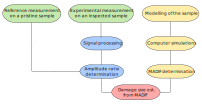
\includegraphics[width=1\linewidth]{Chapter_7/flowchart}
%	%	\end{center}
%	\caption{A flowchart representing the process for damage size estimation.}
%	\label{fig:Flowchart}
%\end{figure}
The \ac{madif} indicates the damage size according to measured damage index \(I\) normalized by the value obtained for the pristine sample \(I^{ref}\).
In the paper, two types of damage index \(I\) are considered: the energy \(I_{eng}\) and the maximum value of the half-width of the first package arrived in the sensor \(I_{amp}\), and these are defined as:
\begin{eqnarray}
	I_{eng}(\Phi_D)=\sum_{t=0}^{T} \left (\Psi_g(t,\Phi_D)\right )^2,\quad I_{eng}^{ref}=\sum_{t=0}^{T} \left (\Psi_g(t,0)\right )^2,\\
	I_{amp}(\Phi_D)=\mathrm{max}\left ( \Psi_g(t,\Phi_D)\right ),\quad I_{amp}^{ref}=\mathrm{max}\left ( \Psi_g(t,0)\right ),
	\label{eq:I_amp}
\end{eqnarray}
where \textit{T} is a period of the signal.
\(\Psi_g(t,\Phi_D)\) is for the damaged case scenario, whereas \(\Psi_g(t,0)\) is for the pristine sample and it is realized in the same way by windowing the full-length signals of the sensor \(\Psi(t)\) with a flattened Gaussian window \emph{g(t)} as follows:
\begin{eqnarray}
	\Psi_g(t)=\Psi(t)g(t)= \Psi(t)\mathrm{exp}\left(-\left(\frac{t-t_0}{0.6005612w_g}\right) ^{12}\right),
	\label{eq:psi_g}
\end{eqnarray}
where \(t_0\) is the center and \(w_g=0.5N_c/f_c\) is a half-width of the window.
Windowing the signals ensures obtaining the signals without any reflections from the boundaries.
The determination of \(\Psi_g\) is pictured in Figure~\ref{fig:window_madif}a.

\begin{figure}[H]
	%	\begin{center}
	\includegraphics[width=1\linewidth]{Chapter_7/window_madif_03}
	%	\end{center}
	\caption{(\textbf{a}) The %MDPI: The hyphen in the picture should be changed to minus sign, e.g., ``-0.5'' to ``$-$0.5'', please change. Please check all like this in all figures. 
		sensor signal \(\Psi(t)\) windowed by a flattened Gaussian window \(g(t)\) and (\textbf{b}) the damage size estimation from the \ac{madif}.}
	\label{fig:window_madif}
\end{figure}
In the time domain, an equivalent numerical signal to the signal registered by the \ac{pzt} acquisition instrument is calculated as an average value of the electrical potential of the electrode surface
\begin{eqnarray}
	\Psi^{n}(t) = \frac{\int_{\Gamma_e}\phi\mathrm{d}\Gamma}{\Gamma_e},
	\label{eq:psi}
\end{eqnarray}
where \(n=1\) and \(n=2\) correspond to the homogenized and presented model, respectively.

The \ac{madif} is achieved by approximating the inverse of the computed damage index that best matches the experimental one.
Finally, the damage size \(\Phi_D\) is obtained from the \ac{madif} curve for measuring the normalized value of \(I/I^{ref}\) as it is presented in Figure~\ref{fig:window_madif}b.
%%% SECTION HEADER /////////////////////////////////////////////////////////////////////////////////////
\section{Determination of the \acs{madif}}
\label{sec:determination}

%% SECTION CONTENT ////////////////////////////////////////////////////////////////////////////////////
The \ac{madif} is determined based on the function best fitted to indices chosen in the previous subsection.
Since the numerically obtained indices take the shape of a non-linear function, several curves were assumed to find the best fit.
These functions are defined in the general form as follows:
\begin{eqnarray}
	y_1(x,a_i) & = & \frac{a_1x}{x+a_2}+a_3,
	\label{eq:function_1}\\
	y_2(x,a_i) & = & a_1\sqrt{x} + a_2x+a_3,
	\label{eq:function_2}\\
	y_3(x,a_i) & = & \frac{a_1x}{\sqrt{a_2 + a_3x^2}}+a_4,\label{eq:function_3} 
\end{eqnarray}
where \(a_i\) are the coefficients of the functions.
The coefficients are determined by built-in function of Matlab named \verb+fminsearch+, which searches for the minimum of a problem specified by \(\min\limits_a f(x,a)\), and the function to be optimised is assumed to be \(f(x,a)=\left\|DI_{num} - y(x,a_i)\right\|\), where \(\left\|\cdot\right\|\) means Euclidean norm.
A criterion for evaluating the fit of the curve to simulation results is a mean absolute error defined as the following:
\begin{eqnarray}
	\delta^{\mathrm{fit}} = \frac{1}{\mathrm{n^{DI}}}\sum_{i=1}^{\mathrm{n^{DI}}} \left|\frac{\mathrm{DI^i_{num}}-y(w_d^i)}{\mathrm{DI^i_{num}}}\right|\times100\%,
\end{eqnarray}
where \(\mathrm{n^{DI}}\) is the number of index points.
The examples of the results for \ac{rmsd} are presented in Tab.~\ref{tab:fit_RMSD_full_FCGM} based on the \ac{fcgm} and in Tab. \ref{tab:fit_RMSD_full_HCGM} for the \ac{hcgm}.
The empty cells in the tables mean that the function has been fitted with an error of more than 20\%.
The \ac{di} is no longer taken into account if the fit function has not been established.
A similar summary has been prepared for the remaining cases, but their presentation has been omitted for chapter clarity.
It turns out that the most fitted function is Eq.~(\ref{eq:function_1}) and Eq.~(\ref{eq:function_2}) for the most \acp{di}.
The best fitted functions were chosen for the \ac{madif} determination.

\begin{table}
	\small
	\tabcolsep=0.1cm
	\centering
	\caption{\label{tab:fit_RMSD_full_FCGM} The errors of the functions fitted to \acf{rmsd} based on full-length windowed signals and the \acf{fcgm}.}
	\begin{tabular}{ccccccccccccccc}
		\toprule
		\multirow{3}{*}{\rotatebox[origin=c]{90}{Frequency}} & \multicolumn{7}{c}{\ac{fcgm} - core} & \multicolumn{7}{c}{\ac{fcgm} - interface}\\
		& \multirow{2}{*}{\rotatebox[origin=c]{90}{DI\(_{num}\)}} & \multicolumn{2}{c}{Eq.~(\ref{eq:function_1})} & \multicolumn{2}{c}{Eq.~(\ref{eq:function_2})} & \multicolumn{2}{c}{Eq.~(\ref{eq:function_3})} &
		\multirow{2}{*}{\rotatebox[origin=c]{90}{DI\(_{num}\)}} & \multicolumn{2}{c}{Eq.~(\ref{eq:function_1})} & \multicolumn{2}{c}{Eq.~(\ref{eq:function_2})} & \multicolumn{2}{c}{Eq.~(\ref{eq:function_3})}\\
		& & \(y(w_d^i)\)& \(\delta^{\mathrm{fit}}\) & \(y(w_d^i)\) & \(\delta^{\mathrm{fit}}\) & \(y(w_d^i)\) & \(\delta^{\mathrm{fit}}\) & & \(y(w_d^i)\)& \(\delta^{\mathrm{fit}}\) & \(y(w_d^i)\) & \(\delta^{\mathrm{fit}}\) & \(y(w_d^i)\) & \(\delta^{\mathrm{fit}}\)\\
		\midrule
		\multirow{7}{*}{\rotatebox[origin=c]{90}{100 \unit{\kHz}}} & 1.00 & 1.00 & \multirow{7}{*}{\rotatebox[origin=c]{90}{\textcolor{green}{1.50}}} & 1.00 & \multirow{7}{*}{\rotatebox[origin=c]{90}{1.70}} & 1.00 & \multirow{7}{*}{\rotatebox[origin=c]{90}{1.92}} & 1.00 & 1.00 & \multirow{7}{*}{\rotatebox[origin=c]{90}{\textcolor{green}{1.11}}} & 1.00 & \multirow{7}{*}{\rotatebox[origin=c]{90}{1.45}} & 1.00 & \multirow{7}{*}{\rotatebox[origin=c]{90}{1.31}} \\
		& 0.83 & 0.85 & & 0.88 & & 0.84 & & 0.92 & 0.92 & & 0.90 & & 0.94 & \\ 
		& 0.82 & 0.80 & & 0.82 & & 0.79 & & 0.85 & 0.84 & & 0.83 & & 0.85 & \\ 
		& 0.80 & 0.78 & & 0.79 & & 0.78 & & 0.79 & 0.79 & & 0.79 & & 0.80 & \\ 
		& 0.76 & 0.78 & & 0.78 & & 0.78 & & 0.76 & 0.77 & & 0.76 & & 0.77 & \\ 
		& 0.77 & 0.77 & & 0.77 & & 0.78 & & 0.73 & 0.75 & & 0.74 & & 0.76 & \\ 
		& 0.75 & 0.77 & & 0.78 & & 0.78 & & 0.75 & 0.73 & & 0.72 & & 0.75 & \\
		\midrule
		\multirow{7}{*}{\rotatebox[origin=c]{90}{150 \unit{\kHz}}} & 1.00 & 1.00 & \multirow{7}{*}{\rotatebox[origin=c]{90}{3.10}} & 1.00 & \multirow{7}{*}{\rotatebox[origin=c]{90}{\textcolor{green}{1.28}}} & 1.00 & \multirow{7}{*}{\rotatebox[origin=c]{90}{6.83}} & 1.00 & 1.00 & \multirow{7}{*}{\rotatebox[origin=c]{90}{1.32}} & 1.00 & \multirow{7}{*}{\rotatebox[origin=c]{90}{\textcolor{green}{0.73}}} & 1.00 & \multirow{7}{*}{\rotatebox[origin=c]{90}{4.85}} \\
		& 0.89 & 0.95 & & 0.92 & & 0.97 & & 0.93 & 0.96 & & 0.95 & & 0.97 & \\ 
		& 0.85 & 0.87 & & 0.85 & & 0.91 & & 0.89 & 0.89 & & 0.88 & & 0.92 & \\ 
		& 0.80 & 0.81 & & 0.79 & & 0.85 & & 0.83 & 0.83 & & 0.82 & & 0.87 & \\ 
		& 0.74 & 0.76 & & 0.74 & & 0.80 & & 0.76 & 0.77 & & 0.77 & & 0.82 & \\ 
		& 0.68 & 0.71 & & 0.70 & & 0.75 & & 0.71 & 0.72 & & 0.72 & & 0.76 & \\ 
		& 0.64 & 0.67 & & 0.65 & & 0.70 & & 0.67 & 0.68 & & 0.67 & & 0.71 & \\ 
		\bottomrule
	\end{tabular}
\end{table}

\begin{table}
	\small
	\tabcolsep=0.1cm
	\centering
	\caption{\label{tab:fit_RMSD_full_HCGM} The errors of the functions fitted to \acf{rmsd} based on full-length windowed signals and the \acf{hcgm}.}
	\begin{tabular}{ccccccccccccccc}
		\toprule
		\multirow{3}{*}{\rotatebox[origin=c]{90}{Frequency}} & \multicolumn{7}{c}{\ac{hcgm} - core} & \multicolumn{7}{c}{\ac{hcgm} - interface}\\
		& \multirow{2}{*}{\rotatebox[origin=c]{90}{DI\(_{num}\)}} & \multicolumn{2}{c}{Eq.~(\ref{eq:function_1})} & \multicolumn{2}{c}{Eq.~(\ref{eq:function_2})} & \multicolumn{2}{c}{Eq.~(\ref{eq:function_3})} &
		\multirow{2}{*}{\rotatebox[origin=c]{90}{DI\(_{num}\)}} & \multicolumn{2}{c}{Eq.~(\ref{eq:function_1})} & \multicolumn{2}{c}{Eq.~(\ref{eq:function_2})} & \multicolumn{2}{c}{Eq.~(\ref{eq:function_3})}\\
		& & \(y(w_d^i)\)& \(\delta^{\mathrm{fit}}\) & \(y(w_d^i)\) & \(\delta^{\mathrm{fit}}\) & \(y(w_d^i)\) & \(\delta^{\mathrm{fit}}\) & & \(y(w_d^i)\)& \(\delta^{\mathrm{fit}}\) & \(y(w_d^i)\) & \(\delta^{\mathrm{fit}}\) & \(y(w_d^i)\) & \(\delta^{\mathrm{fit}}\)\\
		\midrule
		\multirow{7}{*}{\rotatebox[origin=c]{90}{100 \unit{\kHz}}} & 1.00 & 1.00 & \multirow{7}{*}{\rotatebox[origin=c]{90}{\textcolor{green}{5.37}}} & 1.00 & \multirow{7}{*}{\rotatebox[origin=c]{90}{9.85}} & \multirow{7}{*}{-} & \multirow{7}{*}{-} & 1.00 & 1.00 & \multirow{7}{*}{\rotatebox[origin=c]{90}{7.40}} & 1.00 & \multirow{7}{*}{\rotatebox[origin=c]{90}{\textcolor{green}{6.22}}} & 1.00 & \multirow{7}{*}{\rotatebox[origin=c]{90}{11.15}} \\
		& 0.55 & 0.57 & & 0.71 & & & & 0.67 & 0.75 & & 0.74 & & 0.80 & \\ 
		& 0.57 & 0.53 & & 0.58 & & & & 0.61 & 0.57 & & 0.59 & & 0.58 & \\ 
		& 0.57 & 0.52 & & 0.54 & & & & 0.53 & 0.50 & & 0.51 & & 0.51 & \\ 
		& 0.48 & 0.51 & & 0.52 & & & & 0.45 & 0.46 & & 0.46 & & 0.48 & \\ 
		& 0.50 & 0.51 & & 0.53 & & & & 0.35 & 0.44 & & 0.42 & & 0.47 & \\ 
		& 0.47 & 0.51 & & 0.55 & & & & 0.42 & 0.42 & & 0.40 & & 0.46 & \\ 
		\midrule
		\multirow{7}{*}{\rotatebox[origin=c]{90}{150 \unit{\kHz}}} & 1.00 & 1.00 & \multirow{7}{*}{\rotatebox[origin=c]{90}{0.51}} & 1.00 & \multirow{7}{*}{\rotatebox[origin=c]{90}{\textcolor{green}{0.33}}} & 1.00 & \multirow{7}{*}{\rotatebox[origin=c]{90}{2.41}} & 1.00 & 1.00 & \multirow{7}{*}{\rotatebox[origin=c]{90}{\textcolor{green}{0.79}}} & 1.00 & \multirow{7}{*}{\rotatebox[origin=c]{90}{\textcolor{green}{0.79}}} & \multirow{7}{*}{-} & \multirow{7}{*}{-} \\
		& 0.96 & 0.97 & & 0.97 & & 0.98 & & 0.95 & 0.95 & & 0.94 & & & \\ 
		& 0.93 & 0.93 & & 0.93 & & 0.95 & & 0.88 & 0.89 & & 0.89 & & & \\ 
		& 0.89 & 0.89 & & 0.89 & & 0.91 & & 0.84 & 0.85 & & 0.85 & & & \\ 
		& 0.85 & 0.85 & & 0.85 & & 0.88 & & 0.82 & 0.82 & & 0.82 & & & \\ 
		& 0.81 & 0.81 & & 0.81 & & 0.84 & & 0.80 & 0.79 & & 0.79 & & & \\ 
		& 0.77 & 0.78 & & 0.78 & & 0.80 & & 0.76 & 0.77 & & 0.76 & & & \\ 
		\bottomrule
	\end{tabular}
\end{table}

Then all chosen \acp{di} and their fitted functions are compared with experimental results.
The best results were obtained for the \ac{rmsd} and \ac{cc} based on the full-length signals at 100 \unit{kHz}. 
Those indices are presented in Fig.~\ref{fig:madif_rmsd_best} and Fig.~\ref{fig:madif_cc_best}, respectively.
\begin{figure}
	\begin{center}
		\includegraphics[width=0.95\textwidth]{Chapter_7/MADIF_RMSD_100_best_err}
	\end{center}
	\caption{ \textbf{(a)} Comparison of the \acf{madif} based on \acf{rmsd} and the experimental results, and \textbf{(b)} the percentage error between them.}
	\label{fig:madif_rmsd_best}
\end{figure}

\begin{figure}
	\begin{center}
		\includegraphics[width=0.95\textwidth]{Chapter_7/MADIF_CC_100_best_err}
	\end{center}
	\caption{\textbf{(a)} Comparison of the \acf{madif} based on \acf{cc} and the experimental results, and \textbf{(b)} the percentage error between them.}
	\label{fig:madif_cc_best}
\end{figure}
Both indices achieved the lowest error around 5\% for the \ac{fcgm}, with the interface elements removed as the damage model.
The indices are also in very good agreement for the \ac{fcgm} with removed cells as a damage model.
In the case of \ac{hcgm}, unsatisfactory results are obtained, as none of the indices correspond to the experimental ones with an error of less than 20\%.
What may be relevant here is that the wave transmits energy to the core throughout its propagation.
In contrast, in the case of \ac{fcgm}, the wave transmits energy incidentally, encountering cell walls.

According to the analysis, the \ac{rmsd} and \ac{cc} based on \ac{fcgm} and full-length signals at 100 \unit{kHz} were chosen as the \ac{madif}.
From Eq. \ref{eq:function_1}, they are defined as:
\begin{eqnarray}
	MADIF^{RMSD}(w_d) & = & {1.2695w_d}/(w_d+25.4048)+0.95,
	\label{eq:MADIF_RMSD}\\
	MADIF^{CC}(w_d) & = & 1.6091w_d/(w_d+6.6010)+0.7562,
	\label{eq:MADIF_CC}
\end{eqnarray}

The comparison of the \ac{madif} and the \ac{edif} based on \ac{rmsd} and \ac{cc} are presented in Fig.~\ref{fig:madif_20}.
The \ac{edif} was found using the fit function from Eq.~(\ref{eq:function_1}), the same as the \ac{madif}, for the \acp{di} based on experimental measurements.
The \ac{rmsd} is in excellent agreement with experiment, achieving an absolute error of less than 4 mm over the full range of damage.
For the \ac{cc}, the result is not as good as the previous one, but it also agrees with the experiment.
The absolute error is less than 9 mm.
Both indices can be used to estimate the damage size in the assumed scenario with a proposed approximation function.
\begin{figure}[!tbh]
	\begin{center}
		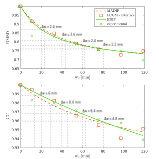
\includegraphics[width=1.0\textwidth]{Chapter_7/MADIF_20}
	\end{center}
	\caption{The \acf{madif} and the \acf{edif} based on the \acf{rmsd} 100 \unit{\kHz}.}
	\label{fig:madif_20}
\end{figure}
\clearpage
%%% SECTION HEADER /////////////////////////////////////////////////////////////////////////////////////
\section{Temperature Compensation}
\label{sec:compensation}

%% SECTION CONTENT ////////////////////////////////////////////////////////////////////////////////////

%%% SECTION HEADER /////////////////////////////////////////////////////////////////////////////////////
\section{Conclusions}
\label{sec:conclusionsSever}

%% SECTION CONTENT ////////////////////////////////////////////////////////////////////////////////////
In the chapter, the \ac{madif} was determined by which the milestone of the dissertation was achieved.
For this purpose, four damage indicators were analysed for two different models of the panel core, two of which proved useless.
From among them, the one that best matched the measurements was selected to determine the function.
The numerical results are in good agreement with the experimental measurements.
It demonstrates the confirmation of the thesis that it is possible to determine the damage severity function in \ac{hsc} by employing numerical simulations.
% Note that the text in the [] brackets is the one that will
% appear in the table of contents, whilst the text in the {}
% brackets will appear in the main thesis.

%% CHAPTER HEADER /////////////////////////////////////////////////////////////////////////////////////
\chapter[Conclusions]{Conclusions}
\label{ch:conclusions}

%% CHAPTER INTRODUCTION ///////////////////////////////////////////////////////////////////////////////



%% INCLUDE SECTIONS ///////////////////////////////////////////////////////////////////////////////////

%% SECTION HEADER /////////////////////////////////////////////////////////////////////////////////////
\section{Concluding remarks}
\label{sec:remarks}

%% SECTION CONTENT ////////////////////////////////////////////////////////////////////////////////////

%% SECTION HEADER /////////////////////////////////////////////////////////////////////////////////////
\section{Contributions}
\label{sec:contributions}

%% SECTION CONTENT ////////////////////////////////////////////////////////////////////////////////////

% Note that the text in the [] brackets is the one that will
% appear in the table of contents, whilst the text in the {}
% brackets will appear in the main thesis.

%% CHAPTER HEADER /////////////////////////////////////////////////////////////////////////////////////

%% CHAPTER INTRODUCTION ///////////////////////////////////////////////////////////////////////////////

\appendix
%% INCLUDE SECTIONS ///////////////////////////////////////////////////////////////////////////////////
% Note that the text in the [] brackets is the one that will
% appear in the table of contents, whilst the text in the {}
% brackets will appear in the main thesis.

%% APPENDIX HEADER ////////////////////////////////////////////////////////////////////////////////////
\chapter{Elementary matrices of the equation of motion.}
\label{app:matrices}
%% APPENDIX CONTENT ///////////////////////////////////////////////////////////////////////////////////

\section{\ac{pzt} matrices}
% start a new page without indent 4.6cm
%\clearpage
The effective properties of the \ac{cfrp} and homogenized honeycomb core are given in Tab.~\ref{tab:properties_eff}.
\vspace{-12pt}
\begin{table}[H]
	%	\centering
	\small
	
	\tabcolsep=0.25cm
	\caption{\label{tab:properties_eff} The effective mechanical properties.}
	\begin{tabular}{ccccccccc}
		\toprule
		\multirow{2}{*}{\textbf{Material}} & $\boldsymbol{E_{11}}$ & $\boldsymbol{E_{22}}$ & $\boldsymbol{E_{33}}$ & $\boldsymbol{G_{12}}$ & $\boldsymbol{G_{23}}$ & $\boldsymbol{\nu_{12}}$	& $\boldsymbol{\nu_{23}}$ & $\boldsymbol{\rho}$ \\
		& \textbf{[GPa]} & \textbf{[GPa]} & \textbf{[GPa]} & \textbf{[GPa]} & \textbf{[GPa]} & \textbf{[--]} & \textbf{[--]} & \textbf{[kg/m}$\boldsymbol{^3}$\textbf{]}\\
		\midrule
		\ac{cfrp} & 137 & 8.7 & 8.7 & 3.61 & 3.19 & 0.28 & 0.37 & 1569\\
		single layer & & & & & & & &\\ \midrule
		aluminium & 40e{$-$6} & 40e{$-$6} & 663e{$-$3} & 24e{$-$6} & 148e{$-$3} & 0.998 & 0.02e{$-$3} & 25.36\\
		honeycomb & & & & & & & &\\
		\bottomrule
	\end{tabular}
\end{table}

% Note that the text in the [] brackets is the one that will
% appear in the table of contents, whilst the text in the {}
% brackets will appear in the main thesis.

%% APPENDIX HEADER ////////////////////////////////////////////////////////////////////////////////////

\chapter{Interfaces coupling matrix}
\label{app:algorithm}

%% APPENDIX CONTENT ///////////////////////////////////////////////////////////////////////////////////
% Note that the text in the [] brackets is the one that will
% appear in the table of contents, whilst the text in the {}
% brackets will appear in the main thesis.

%% APPENDIX HEADER ////////////////////////////////////////////////////////////////////////////////////
\chapter[Appendix 3]{Appendix 3}
\label{appc}

%% APPENDIX CONTENT ///////////////////////////////////////////////////////////////////////////////////

\lipsum[1]


% A small file that prints the index in the main document.
% No need to alter this file...
\printindex


% Bibliography
\addcontentsline{toc}{chapter}{References/Bibliography}
\printbibliography

\end{document}
